\documentclass[hyperref=colorlinks]{beamer}
\mode<presentation>
\usetheme{iclpt}
\setbeamertemplate{navigation symbols}{}
\setbeamertemplate{headline}{
  \begin{beamercolorbox}[leftskip=.2cm,rightskip=.2cm,topskip=.2cm,ht=1.1cm,dp=0.1cm,wd=\textwidth]{institute in head/foot}
    
\includegraphics[height=1cm]{icl.pdf}
    \hfill
    
\includegraphics[height=1cm]{../Pics/CMS-Color.pdf}
  \end{beamercolorbox}
}
\setbeamertemplate{footline}{
  \begin{beamercolorbox}[ht=.35cm,dp=0.2cm,wd=\textwidth,leftskip=.3cm]{author in head/foot}%
    \begin{minipage}[c]{5cm}%
      \usebeamerfont{author in head/foot}
      \insertshortauthor 
      \insertshorttitle
    \end{minipage}\hfill%
    \hfill
    \insertframenumber{} / \pageref{lastframe}
    %\hfill
    \begin{minipage}{6cm}
      \hfill
      %\insertshorttitle
    \end{minipage}
  \end{beamercolorbox}%
}

\usepackage{tikz}
\usetikzlibrary{arrows,shapes,backgrounds}
\usepackage{color}
\usepackage{tabularx,colortbl}
\usepackage{graphicx}
\usepackage{pdfpages}
\usepackage{feynmp}
\usepackage{rotating}
\usepackage{moresize}
\usepackage{xcolor,colortbl}
\DeclareGraphicsRule{*}{mps}{*}{}

\definecolor{beamer@icdarkblue}{RGB}{0,51,102}
\definecolor{beamer@icmiddleblue}{RGB}{0,82,150}
\definecolor{beamer@iclightblue}{RGB}{200,212,232}
\definecolor{beamer@icmiddlered}{RGB}{204,51,0}
\definecolor{beamer@iclightred}{RGB}{232,212,32}

\title[Invisible Higgs at CMS]{\vspace{-0.2cm} Searches for invisible decays of the Higgs boson with the CMS detector}
\author[P. Dunne]{\underline{P. Dunne} - Imperial College London \\ on behalf of the CMS Collaboration \\ IOP 2015} % A.M. Magnan and A. Nikitenko Joao Pela with \\ R. Aggleton, J. Brooke: Bristol \\ C.Asawangtrakuldee, Q.Li: Peking \\ P. Srimanobhas: Chulalongkorn \\ S. Kumar, K. Mazumdar: Mumbai}
\titlegraphic{
  \vspace{-0.7cm}
  %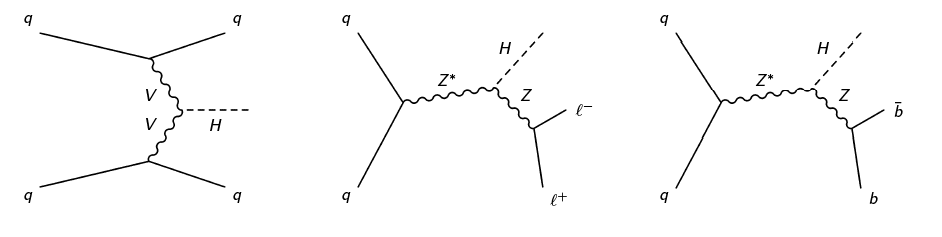
\includegraphics[width=\textwidth]{../invisible/TalkPics/invcomb021213/feyndiags}
  \begin{fmfgraph*}(100,70)
          \fmfleft{i1,i2}
          \fmfright{o1,o2,o3}
          \fmf{fermion}{i1,v1,o1}
          \fmf{fermion}{i2,v2,o3}
          \fmf{phantom,tension=4/5}{v1,v2}
          \fmffreeze
          \fmf{photon,label=$W,,Z$}{v1,v3}
          \fmf{photon,label=$W,,Z$}{v2,v3}
          \fmf{dashes}{v3,o2}
          \fmflabel{$q$}{i1}
          \fmflabel{$q$}{i2}
          \fmflabel{$q$}{o1}
          \fmflabel{$q$}{o3}
          \fmflabel{$H$}{o2}

        \end{fmfgraph*}
}
\date{}
\begin{document}
\tikzstyle{every picture}+=[remember picture]
\tikzstyle{na} = [baseline=-.5ex]
\begin{fmffile}{trfeynmandiags}

  %TITLE PAGE
  \section{Title}
  \begin{frame}
    \titlepage
    
  \end{frame}

\begin{frame}
  \frametitle{My thesis outline}
  \begin{itemize}
  \item Theory
  \item Detector \& physics objects
  \item Statistics
  \item CMS Prompt Higgs to invisible search
  \item CMS Parked Higgs to invisible search
  \item Combination with other searches
  \item Dark matter interpretrations
  \item Run II
  \end{itemize}
\end{frame}

\begin{frame}
  \frametitle{Theory: Why look for invisibly decaying Higgs bosons?}
  \begin{columns}
    \column{.5\textwidth}
    \begin{itemize}
    \item Introduce Standard Model Higgs mechanism
    \item Introduce Dark Matter
    \item Discuss why Higgs is a good place to look for dark matter
    \item[-] Give model examples e.g. EFT, simplified models
    \item Discuss Higgs production and why VBF
    \end{itemize}
    \column{.5\textwidth}
    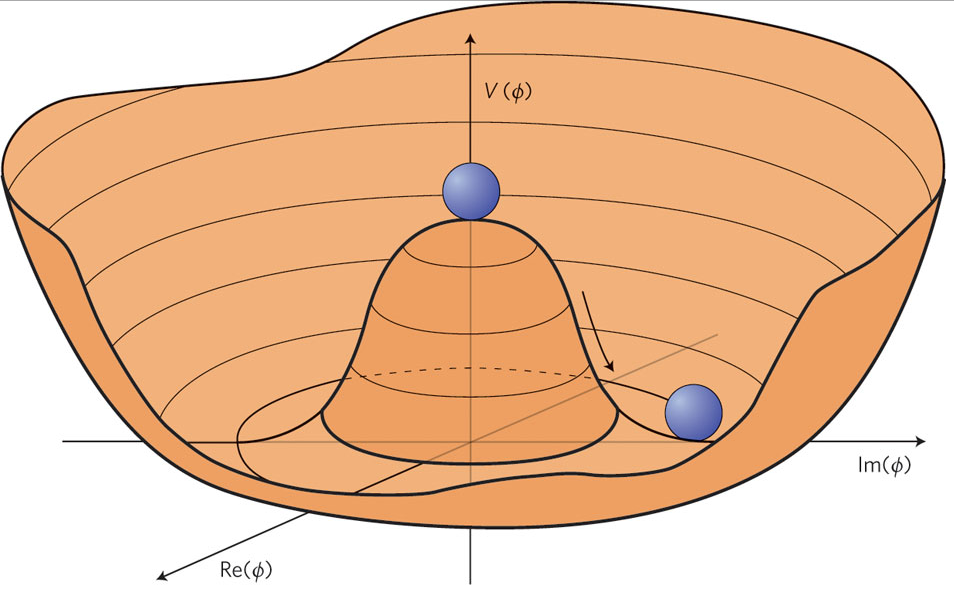
\includegraphics[width=\textwidth]{../invisible/TalkPics/sgs120315/higgspotential.png}
  \end{columns}
\end{frame}

\begin{frame}
    \frametitle{Why look for invisibly decaying Higgs bosons?}
    \begin{columns}
      \column{1.1\textwidth}
    \begin{itemize}
    \item SM compatible 125 GeV Higgs boson observed by ATLAS and CMS
      \begin{itemize}
      \item SM compatible does not mean BSM incompatible
        \end{itemize}
    \end{itemize}
    \end{columns}
    \begin{columns}
      \column{.51\textwidth}
      \begin{columns}
      \column{.9\textwidth}

      \hfill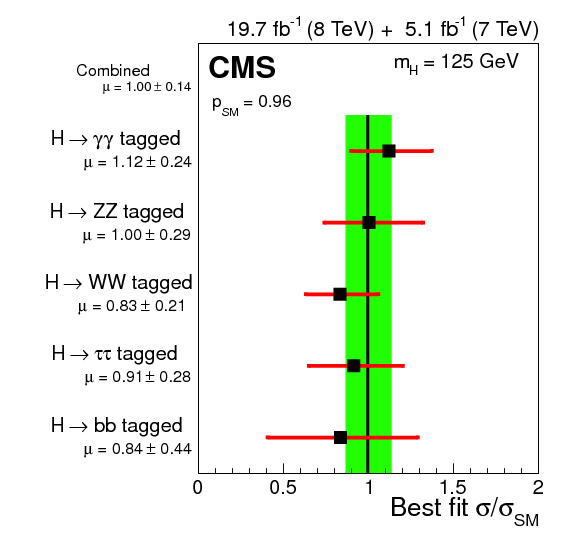
\includegraphics[height=.55\textheight]{../invisible/TalkPics/IOP2015/decaylimits.png}
      \column{.1\textwidth}
      \begin{turn}{-90}\scriptsize CMS-HIG-14-009\end{turn}
%      \column{.45\textwidth}

%      \hfill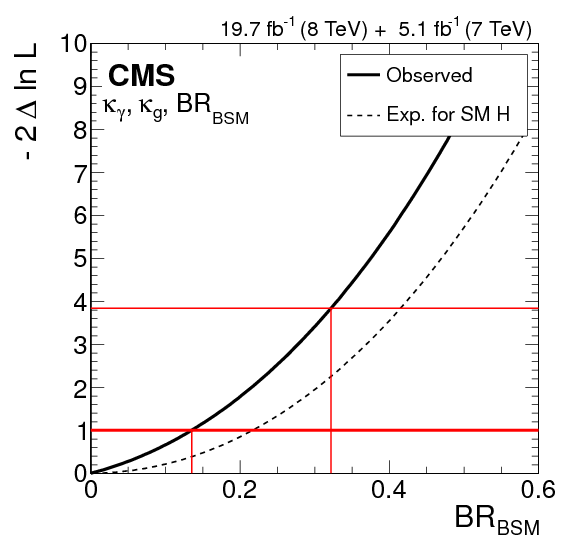
\includegraphics[height=.55\textheight]{../invisible/TalkPics/IOP2015/brbsm.png}
%      \column{.05\textwidth}
%      \begin{turn}{-90}\scriptsize CMS-HIG-14-009\end{turn}
        \end{columns}
    \end{columns}
    \begin{columns}
      \column{1.1\textwidth}
        \begin{itemize}
        \item Many BSM theories predict Higgs to invisible, e.g. SUSY
          \begin{itemize}
          \item Often provide good DM candidates
          \end{itemize}
        \end{itemize}
    \end{columns}

  \end{frame}

\begin{frame}
  \frametitle{Detector \& physics objects}
  %CMS DETECTOR
  \begin{itemize}
  \item LHC overview, introduction to CMS subsystems and objects
  \end{itemize}
  \centering
    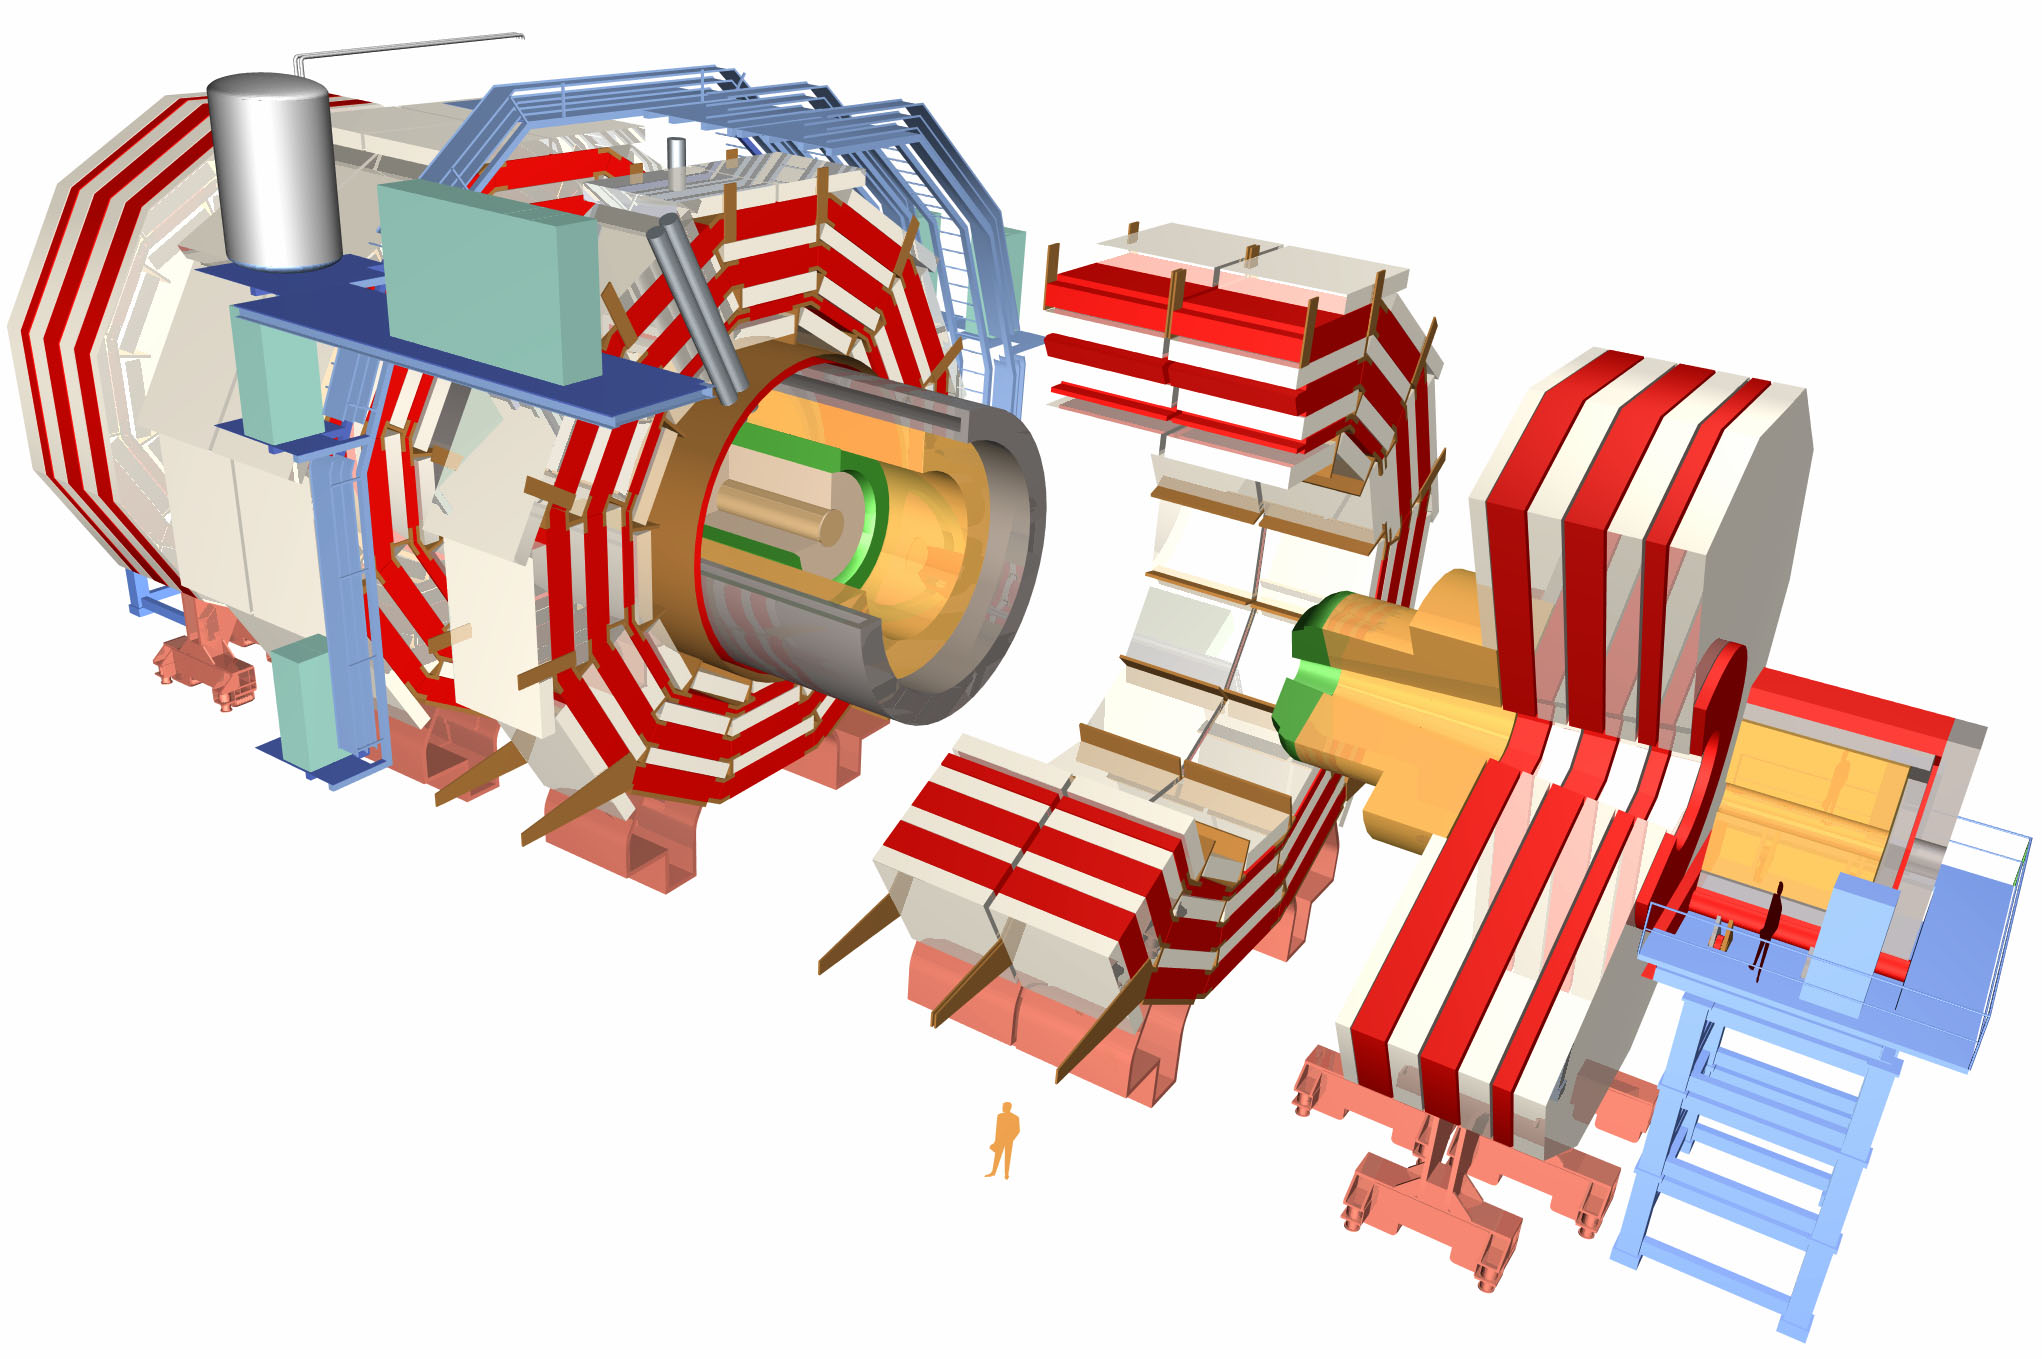
\includegraphics[width=.9\textwidth]{../invisible/TalkPics/IOP2015/CMSdiag.jpg}
\end{frame}

  \begin{frame}
    \frametitle{Invisible signatures at CMS}
    \begin{columns}
      \column{1.1\textwidth}
      \vspace{-.3cm}
      \begin{itemize}
      \item Which signatures do we see at CMS?
      \item Indirect: Look for effect of BSM Higgs decays on Higgs total width
      \item Direct: Use channels where the Higgs recoils against a visible system
        \begin{itemize}
        \item[] \tikz[na] \node (ggH) {ggH: high rate, no visible products (unless ISR/FSR, i.e. mono-X)};        
        \item[] \tikz[na] \node (VBF) {VBF: medium rate, jets+MET final state};        
        \item[] \tikz[na] \node (ZH) {ZH: low rate, leptons/b jets+MET final state};        
        \end{itemize}
      \end{itemize}
    \end{columns}

    \begin{columns}

        \column{.5\textwidth}
%        \tikzstyle{background grid}=[draw, black!50,step=.5cm]
           \begin{tikzpicture}%[show background grid]
            \node [inner sep=0pt,above right]
            {\includegraphics[height=.45\textheight,width=.9\textwidth]{../../Reports/Firstyearreport/Higgs_XS_8TeV_lx.pdf}};
 %           \fill (0,0) circle (2pt);

            \path (1.2,3.1) coordinate (ggHl)
                  (1.9,2.2) coordinate (VBFl)
                  (2.6,1.2) coordinate (ZHl);
          \end{tikzpicture}

          \column{.5\textwidth}
        \centering
        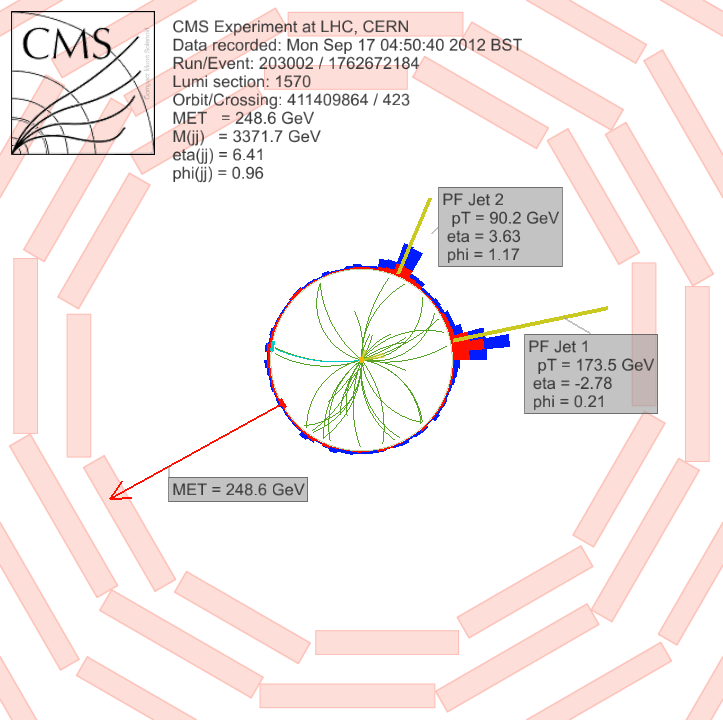
\includegraphics[height=.45\textheight,width=.7\textwidth]{../invisible/TalkPics/sgs120315/vbfevent.png}
      \end{columns}

    \begin{tikzpicture}[overlay]
      \path[->,blue,thick] (ggH.west) edge [bend right] (ggHl);
      \path[->,red,thick] (VBF.west) edge [bend right] (VBFl);
      \path[->,green,thick] (ZH.south) edge [bend left] (ZHl);

    \end{tikzpicture}
  \end{frame}

\begin{frame}
  \frametitle{Statistics}
  \begin{itemize}
  \item A lot of my work has involved limit setting
  \item[-] Short chapter with theory of CLs, nuisance parameter treatment etc.
  \end{itemize}
  \centering
  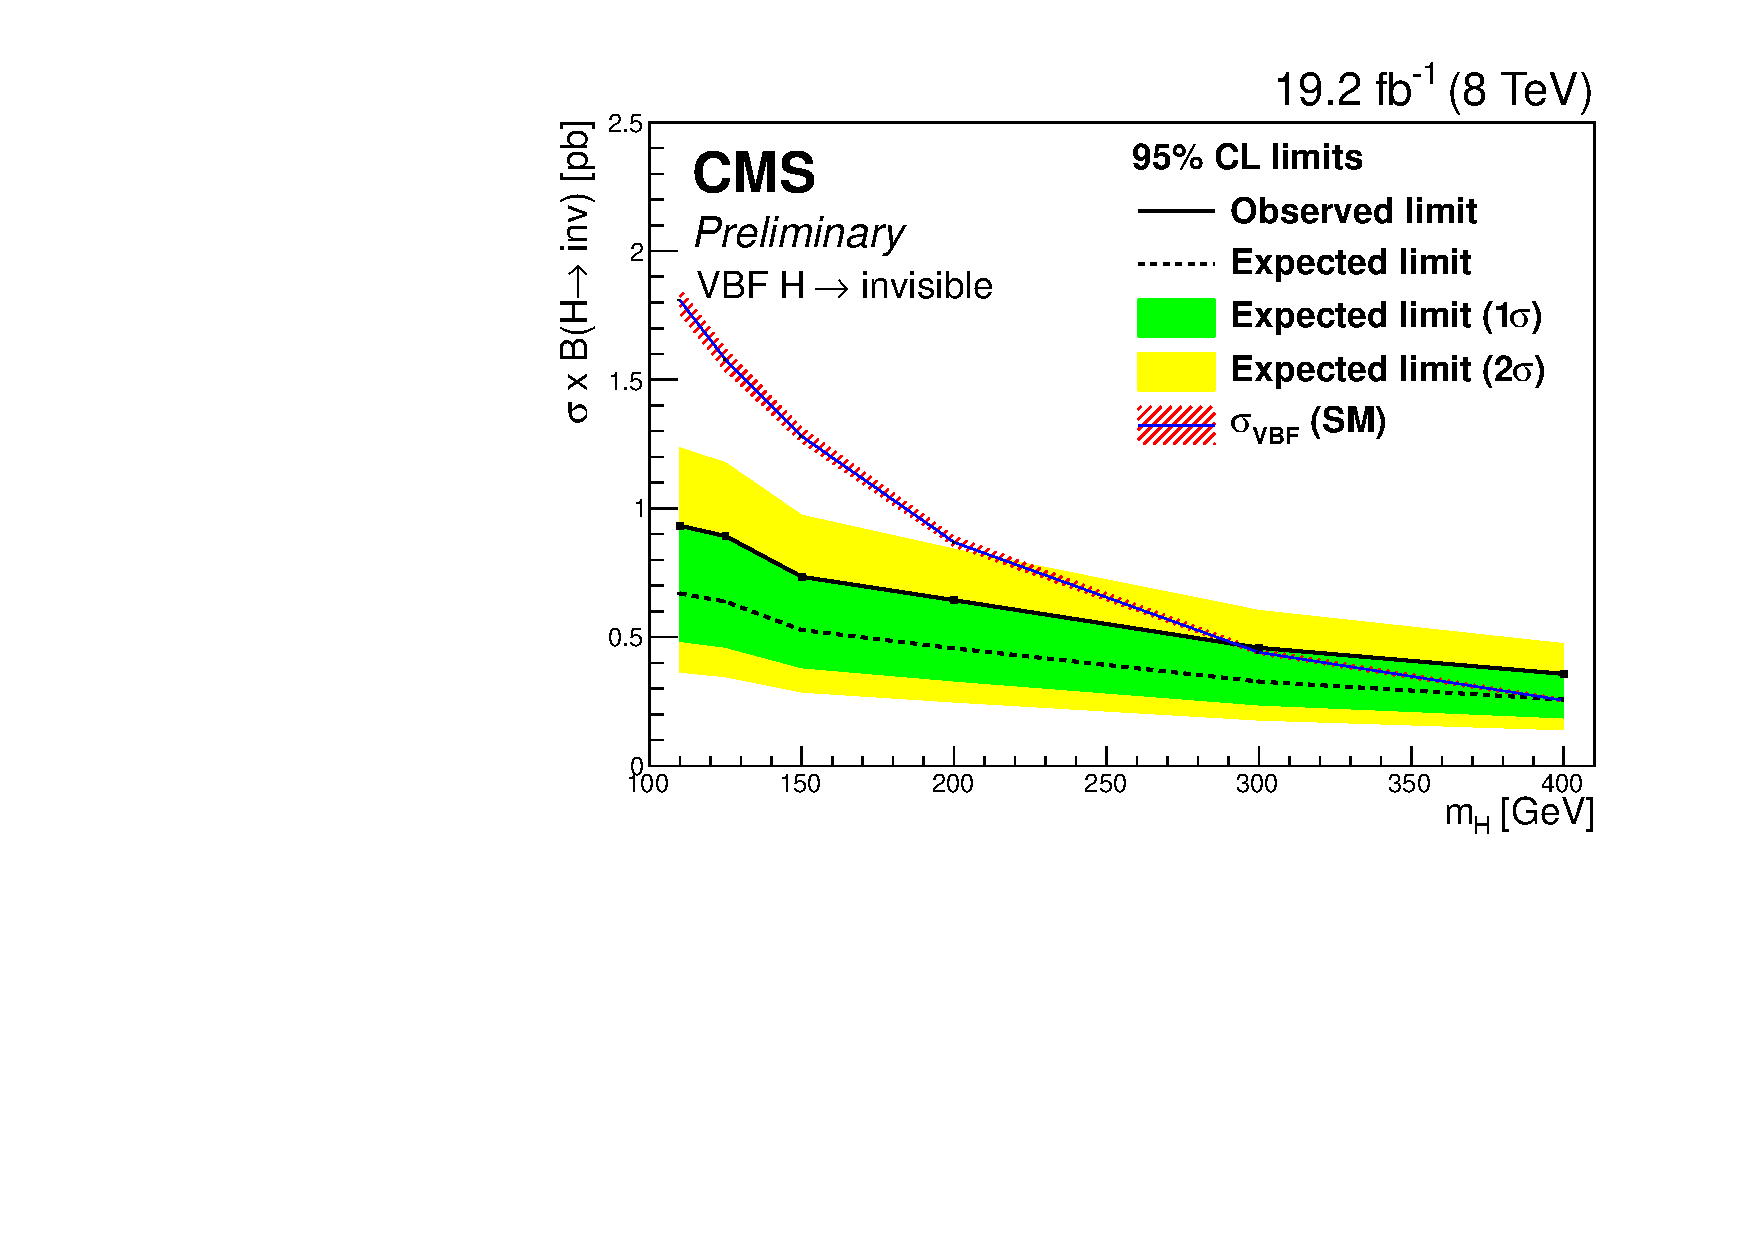
\includegraphics[clip=true,trim=0 0 0 0,width=.55\textwidth]{../invisible/TalkPics/IOP2015/vbfxslimit.pdf}  
\end{frame}

%!!ADD MY CONTRIBUTION TO EACH
\begin{frame}
  \frametitle{CMS VBF History}
  \begin{itemize}
  \item CMS ran two sets of triggers in 2012:
    \begin{itemize}
    \item prompt: reconstructed immediately
    \item parked: looser thresholds, reconstructed in long shutdown
    \end{itemize}
  \item CMS published result using full run I prompt dataset
    \begin{itemize}
    \item I did the limit setting and worked on the cross-check
    \end{itemize}
  \item A CMS PAS was produced using the full run I parked dataset
    \begin{itemize}
    \item I was the main analysis contact
    \item This will be the main piece of work in my thesis
    \end{itemize}
  \end{itemize}
\end{frame}

\begin{frame}
  \frametitle{Prompt VBF}
  \begin{columns}
    \column{.65\textwidth}
    \begin{itemize}
    \item Introduce analysis focusing on my work
    \item[-] Background estimation, systematics, limits
    \end{itemize}
      %\item Restricted phase space necessitates data driven background estimation
    \column{.4\textwidth}
    \begin{fmfgraph*}(100,70)
      \fmfleft{i1,i2}
      \fmfright{o1,o2,o3}
      \fmf{fermion}{i1,v1,o1}
      \fmf{fermion}{i2,v2,o3}
      \fmf{phantom,tension=4/5}{v1,v2}
      \fmffreeze
      \fmf{photon,label=$W,,Z$}{v1,v3}
      \fmf{photon,label=$W,,Z$}{v2,v3}
      \fmf{dashes}{v3,o2}
      \fmflabel{$q$}{i1}
      \fmflabel{$q$}{i2}
      \fmflabel{$q$}{o1}
      \fmflabel{$q$}{o3}
      \fmflabel{$H$}{o2}
      
    \end{fmfgraph*}
    
  \end{columns}
\end{frame}

\begin{frame}
  \frametitle{Parked data VBF analysis}
    \begin{itemize}
    \item I was the main contact for this analysis and it will be the main piece of work in my thesis
    \item Analysis reoptimised using new variables
    \item[-] Target significant MET away from jets
    \item Trigger efficiency remeasured
    \item[-] 3D characterisation to enable trigger turn on to be used
    \item Systematics and background estimations improved

    \end{itemize}
\end{frame}

\begin{frame}
  \frametitle{Parked Triggers}
  \vspace{-.2cm}
    \begin{itemize}
    \item Parked triggers present for runs B, C and D
    \item[-] Parked trigger cuts are looser so prompt trigger not used where parked trigger is available
    \item[-] Two different triggers, one in runs B and C one in run D
    \item Looser thresholds allowed us to look at new regions of phase space and different analysis techniques
    \end{itemize}
  \vspace{-.2cm}
  \begin{block}{\scriptsize HLT}
    \scriptsize
    \centering
    \begin{tabular}{|l|c|c|c|}
      \hline
      Run period & MET cut & dijet $p_{T}$ cut & dijet mass cut \\
      \hline
      A & METnoMuons$>$65 GeV & DiPFJet40 & MJJ800 \\
      B\&C & N/A & DiJet35 & MJJ700 \\
      D & N/A & DiJet30 & MJJ700 \\
      \hline
    \end{tabular}
  \end{block}
\end{frame}

\begin{frame}
  \frametitle{Trigger efficiency}
  \begin{columns}
    \column{.55\textwidth}
      \begin{itemize}
      \item Variables used in triggers are highly correlated
      \item In prompt analysis correlations neglected
      \item[-] cut tighter to ensure trigger is efficient
      \item For the parked analysis fit trigger turn on in each bin of a 2D grid
      \item[-] Cuts can then be looser

      \end{itemize}
    \column{.5\textwidth}
    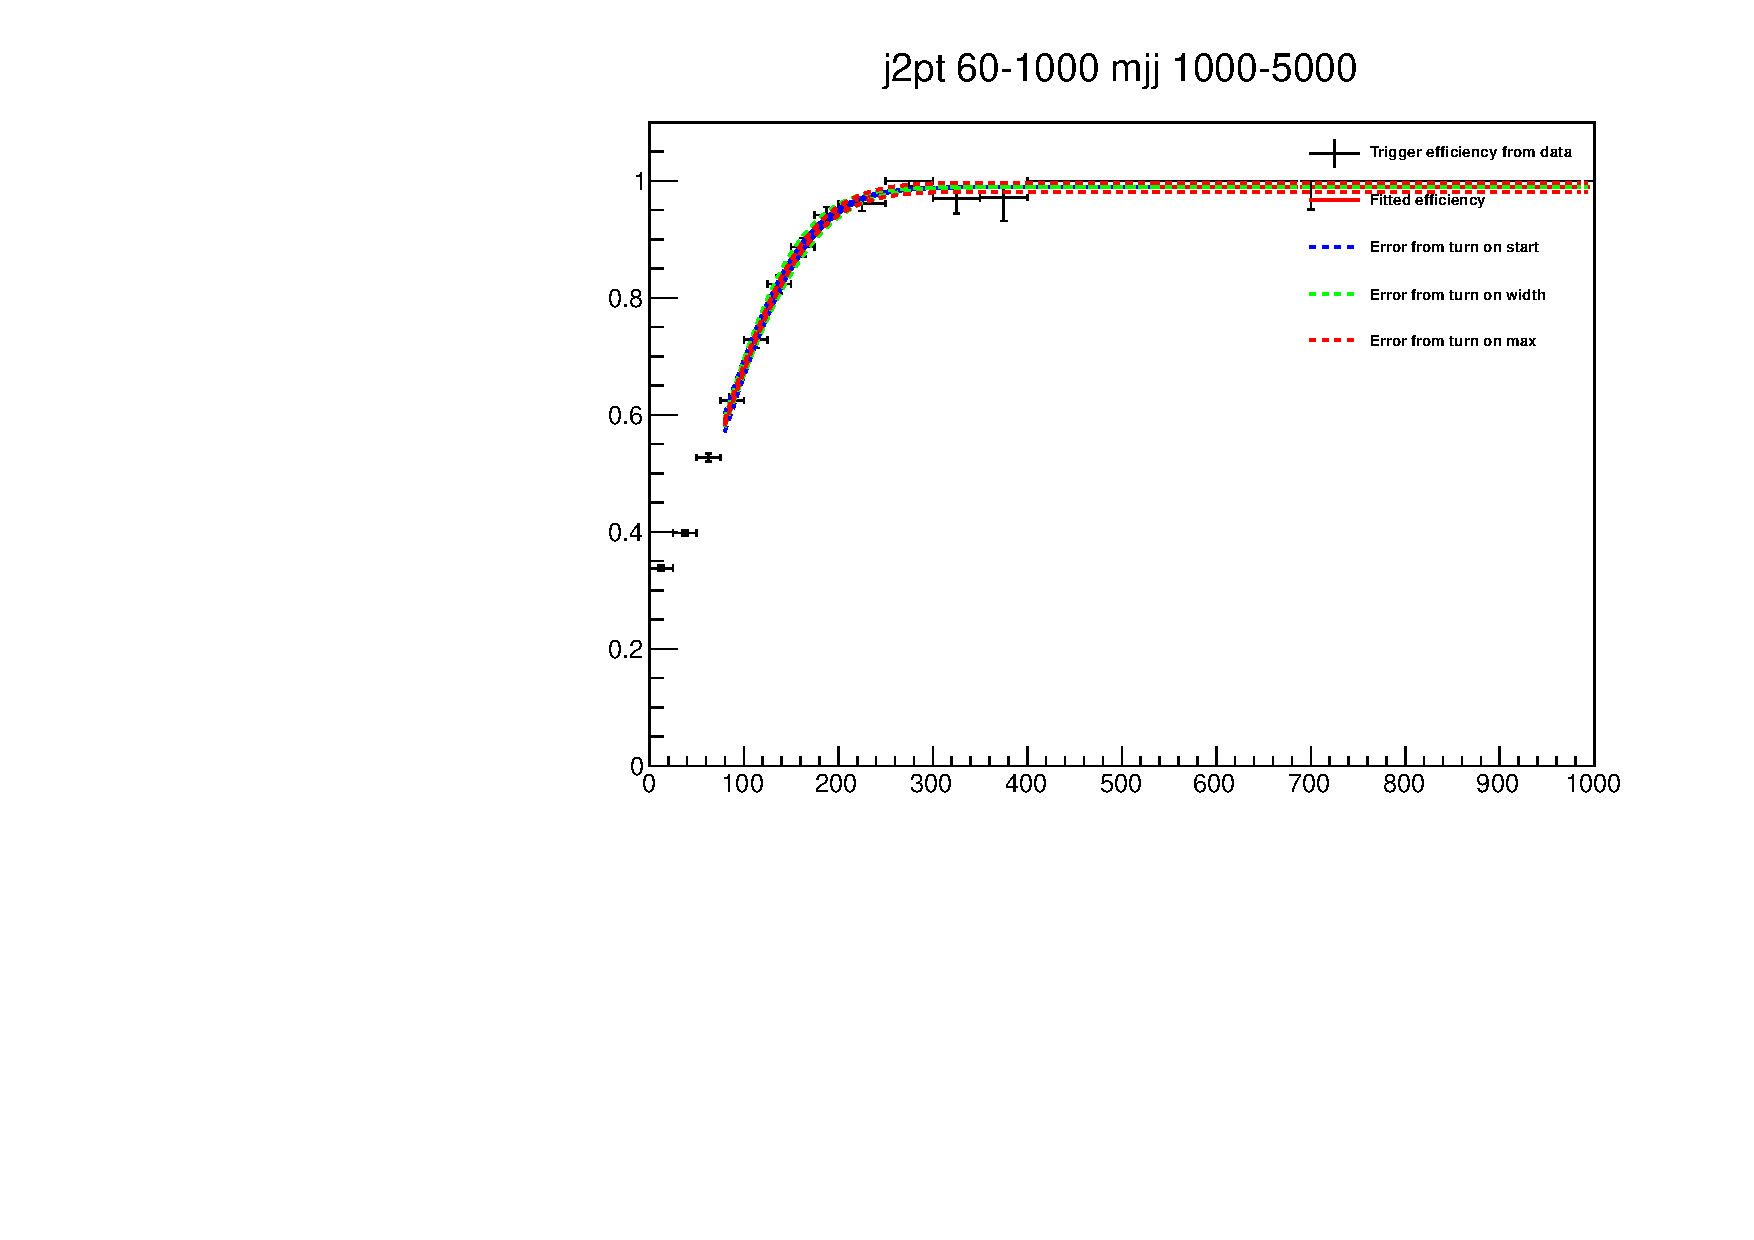
\includegraphics[width=1.1\textwidth]{../invisible/TalkPics/hig14038preapproval/trigfitplots/hData_MET_1D_45D.pdf}
    \vspace{-.2cm}

    \hfill \scriptsize METnoMU/GeV
  \end{columns}
\end{frame}

\begin{frame}
  \frametitle{VBF: selection}
  \vspace{.5cm}
  \begin{itemize}
    \item Select events with two VBF jets
      + MET:
      \begin{itemize}
      \item no colour connection between jets means large $\eta$ gap
      \end{itemize}
    \item QCD background difficult to model:
      \begin{itemize}
      \item use tight selection to remove
      \end{itemize}
  \item Main backgrounds: $W\rightarrow\ell\nu/Z\rightarrow\nu\nu$+jets, QCD, top
    \begin{itemize}
    \item Veto events with leptons present
      %\item Require MET to be significant compared to event activity
    \end{itemize}
  \end{itemize}
  \begin{columns}
    \column{.3\textwidth}
    \begin{block}{W+jets}
      %WJETS                                                                                                                                                  
      \centering           
      \begin{fmfgraph*}(45,60)
        \fmftop{i1,m1,m2,o1}
        \fmfbottom{i2,o2}
        \fmf{fermion,label=$e/\mu/\tau$,label.side=left}{v2,m1}
        \fmf{fermion,label=$\nu$,label.side=right}{v2,m2}
        \fmf{photon,tension=7/5,label=$W$}{v1,v2}
        \fmf{fermion}{v1,i2}
        \fmf{fermion}{v1,o2}
        \fmflabel{$jet$}{i2}
        \fmflabel{$jet$}{o2}
      \end{fmfgraph*}
      \vspace{.3cm}
    \end{block}
    \column{.3\textwidth}
    \begin{block}{Z+jets}
      %ZJETS                                                                                                                                                                     
      \centering
      \begin{fmfgraph*}(45,60)
        \fmftop{i1,m1,m2,o1}
        \fmfbottom{i2,o2}
        \fmf{fermion}{v1,i2}
        \fmf{fermion}{v1,o2}
        \fmf{photon,tension=7/5,label=$Z$}{v1,v2}
        \fmf{fermion,label=$\nu$,label.side=left}{v2,m1}
        \fmf{fermion,label=$\nu$,label.side=right}{v2,m2}
        \fmflabel{$jet$}{i2}
        \fmflabel{$jet$}{o2}
      \end{fmfgraph*}
      \vspace{.3cm}
    \end{block}
    \column{.3\textwidth}
    \begin{block}{QCD}
      %QCD                                                                                                                                                                
      \centering
      \begin{fmfgraph*}(45,60)
        \fmftop{i1,m1,m2,m3,m4,o1}
        \fmfbottom{i2,o2}
        \fmf{fermion,tension=4}{v1,i2}
        \fmf{fermion,tension=4}{v1,o2}
        \fmf{fermion,label=$jets$,label.side=left}{v1,m1}
        \fmf{fermion}{v1,m2}
        \fmf{fermion}{v1,m3}
        \fmf{fermion}{v1,m4}
        \fmflabel{$jet$}{i2}
        \fmflabel{$jet$}{o2}
      \end{fmfgraph*}
      \vspace{.3cm}
    \end{block}
    
  \end{columns}
\end{frame}

  \begin{frame}
    \frametitle{VBF: background estimation}
    \vspace{-.15cm}
    \begin{itemize}
    \item All major backgrounds have data driven normalisation
    \vspace{-.2cm}
      \begin{block}{}
        \centering
      $N_{bkg}^{sig}=\frac{(N_{obs}^{control}-N_{other\,bkgs}^{control})}{N_{MC}^{control}}\cdot N_{MC}^{sig}$
        \end{block}
    \item Most backgrounds from missed lepton or misreconstructed jet
      \begin{itemize}
      \item use control region where object is reconstructed
      \end{itemize}
    \end{itemize}

    \begin{columns}
      \column{.03\textwidth}
      \column{.55\textwidth}
        $W\rightarrow\mu\nu$ control region
      \begin{columns}
        \column{.9\textwidth}
      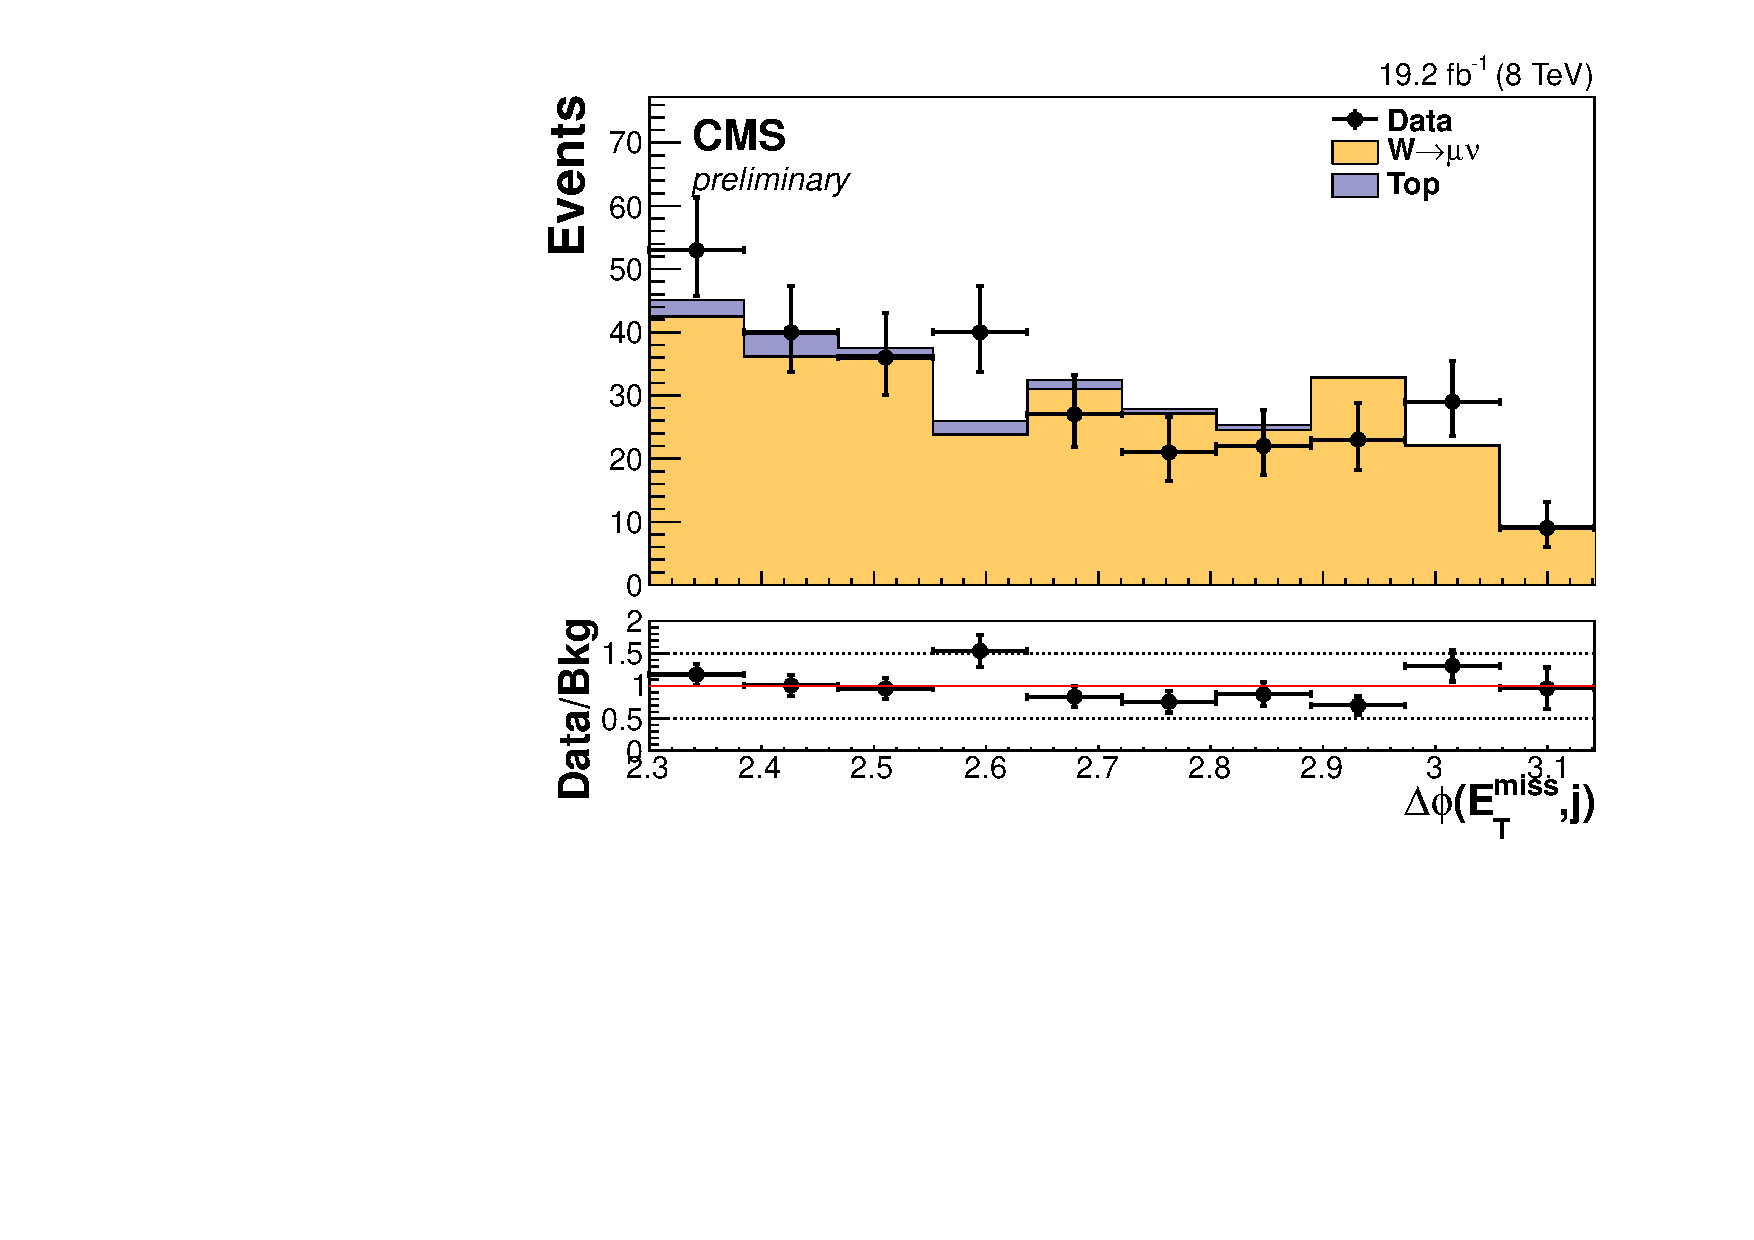
\includegraphics[clip=true,trim=0 0 0 0,width=1.1\textwidth]{../invisible/TalkPics/IOP2015/output_sigreg/munu_alljetsmetnomu_mindphi.pdf}
      \column{.1\textwidth}
      \hspace{-.5cm}
      \begin{turn}{-90}\scriptsize CMS-PAS-HIG-14-038 \end{turn}
      \end{columns}
      \column{.55\textwidth}
        $Z\rightarrow\nu\nu$ control region
      \begin{columns}
        \column{.9\textwidth}
      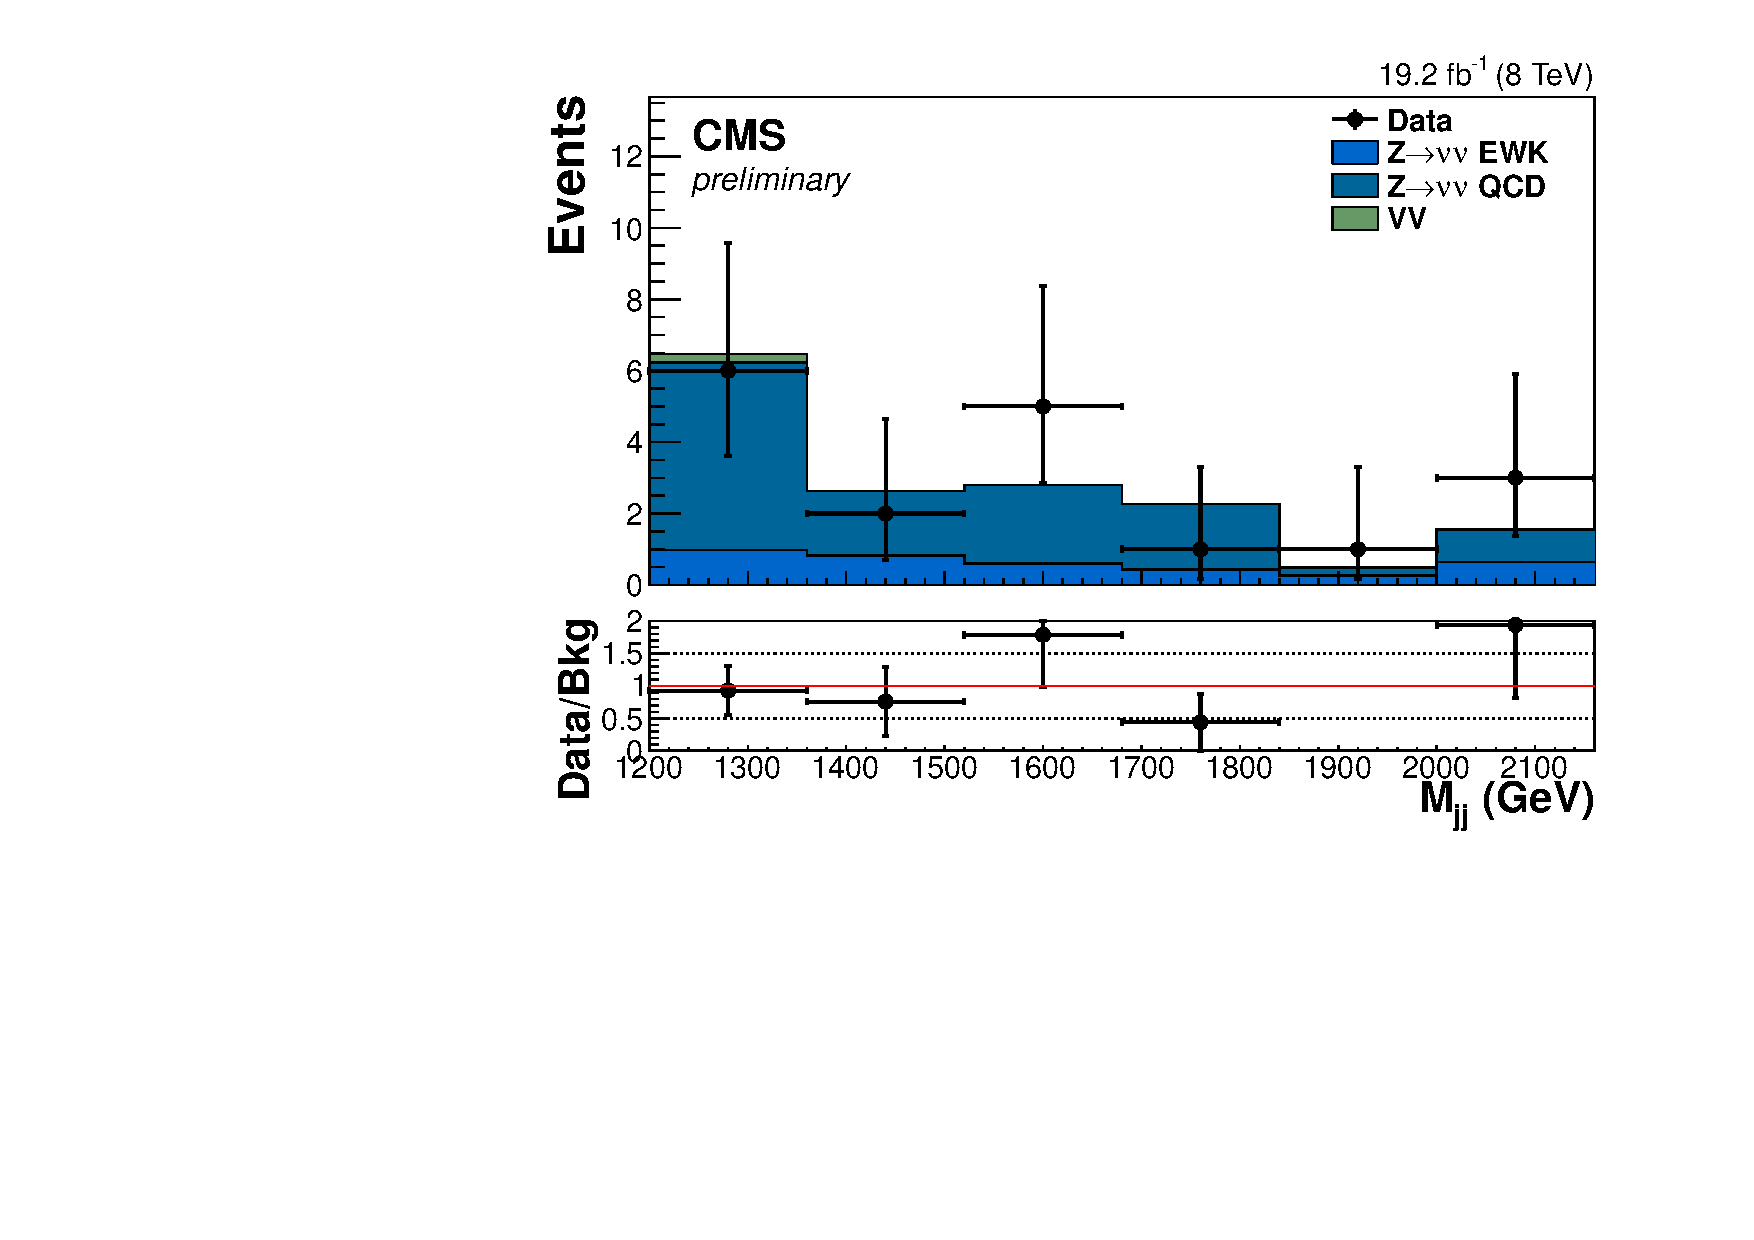
\includegraphics[clip=true,trim=0 0 0 0,width=1.1\textwidth]{../invisible/TalkPics/IOP2015/output_sigreg/mumu_dijet_M.pdf}
      \column{.1\textwidth}
      \hspace{-.5cm}
      \begin{turn}{-90}\scriptsize CMS-PAS-HIG-14-038 \end{turn}
      \end{columns}
    \end{columns}
  \end{frame}

  \begin{frame}
    \frametitle{VBF results}
          \scriptsize
          \centering
          \begin{tabular}{lc}
            \hline
            Total background & $439.7\pm 41.0 (stat.) \pm 55.8 (syst.)$ \\ 
            \hline
            VBF H(inv.) assuming B(H$\rightarrow$inv)=100\% &  $273.4 \pm 31.2(syst.)$ \\ 
            ggF H(inv.) assuming B(H$\rightarrow$inv)=100\%& $22.6 \pm 15.6 (syst.)$ \\
            \hline
            Observed data & 508 \\
            \hline
          \end{tabular}
          \normalsize
    \begin{itemize}
    \item Compatible with the background hypothesis
    \end{itemize}
    \begin{columns}
      \column{.03\textwidth}
      \column{.55\textwidth}
      Signal region
      \begin{columns}
        \column{.9\textwidth}
      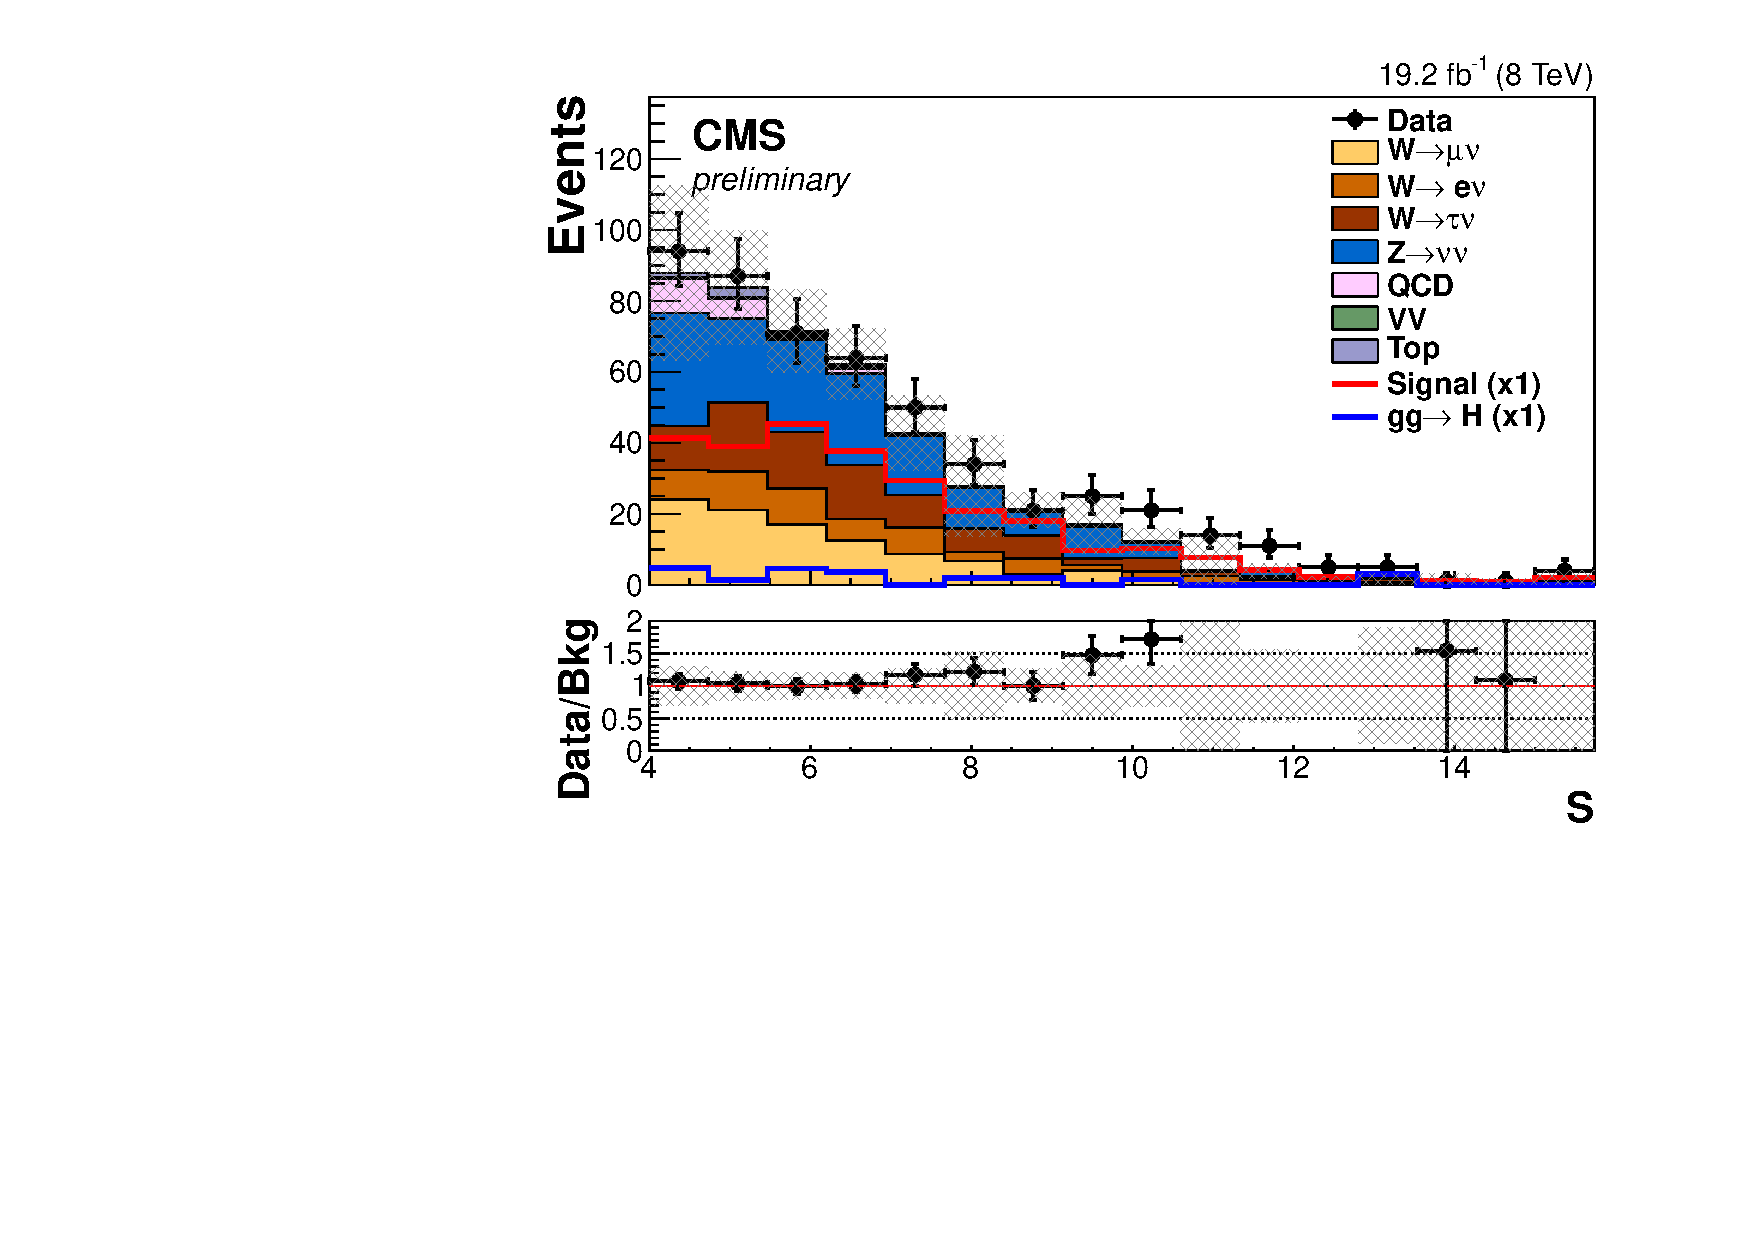
\includegraphics[clip=true,trim=0 0 0 0,width=1.1\textwidth]{../invisible/TalkPics/IOP2015/output_sigreg/nunu_metnomu_significance.pdf}
      \column{.1\textwidth}
      \hspace{-.5cm}
      \begin{turn}{-90}\scriptsize CMS-PAS-HIG-14-038 \end{turn}
      \end{columns}
      \column{.55\textwidth}
      Signal region
      \begin{columns}
        \column{.9\textwidth}
      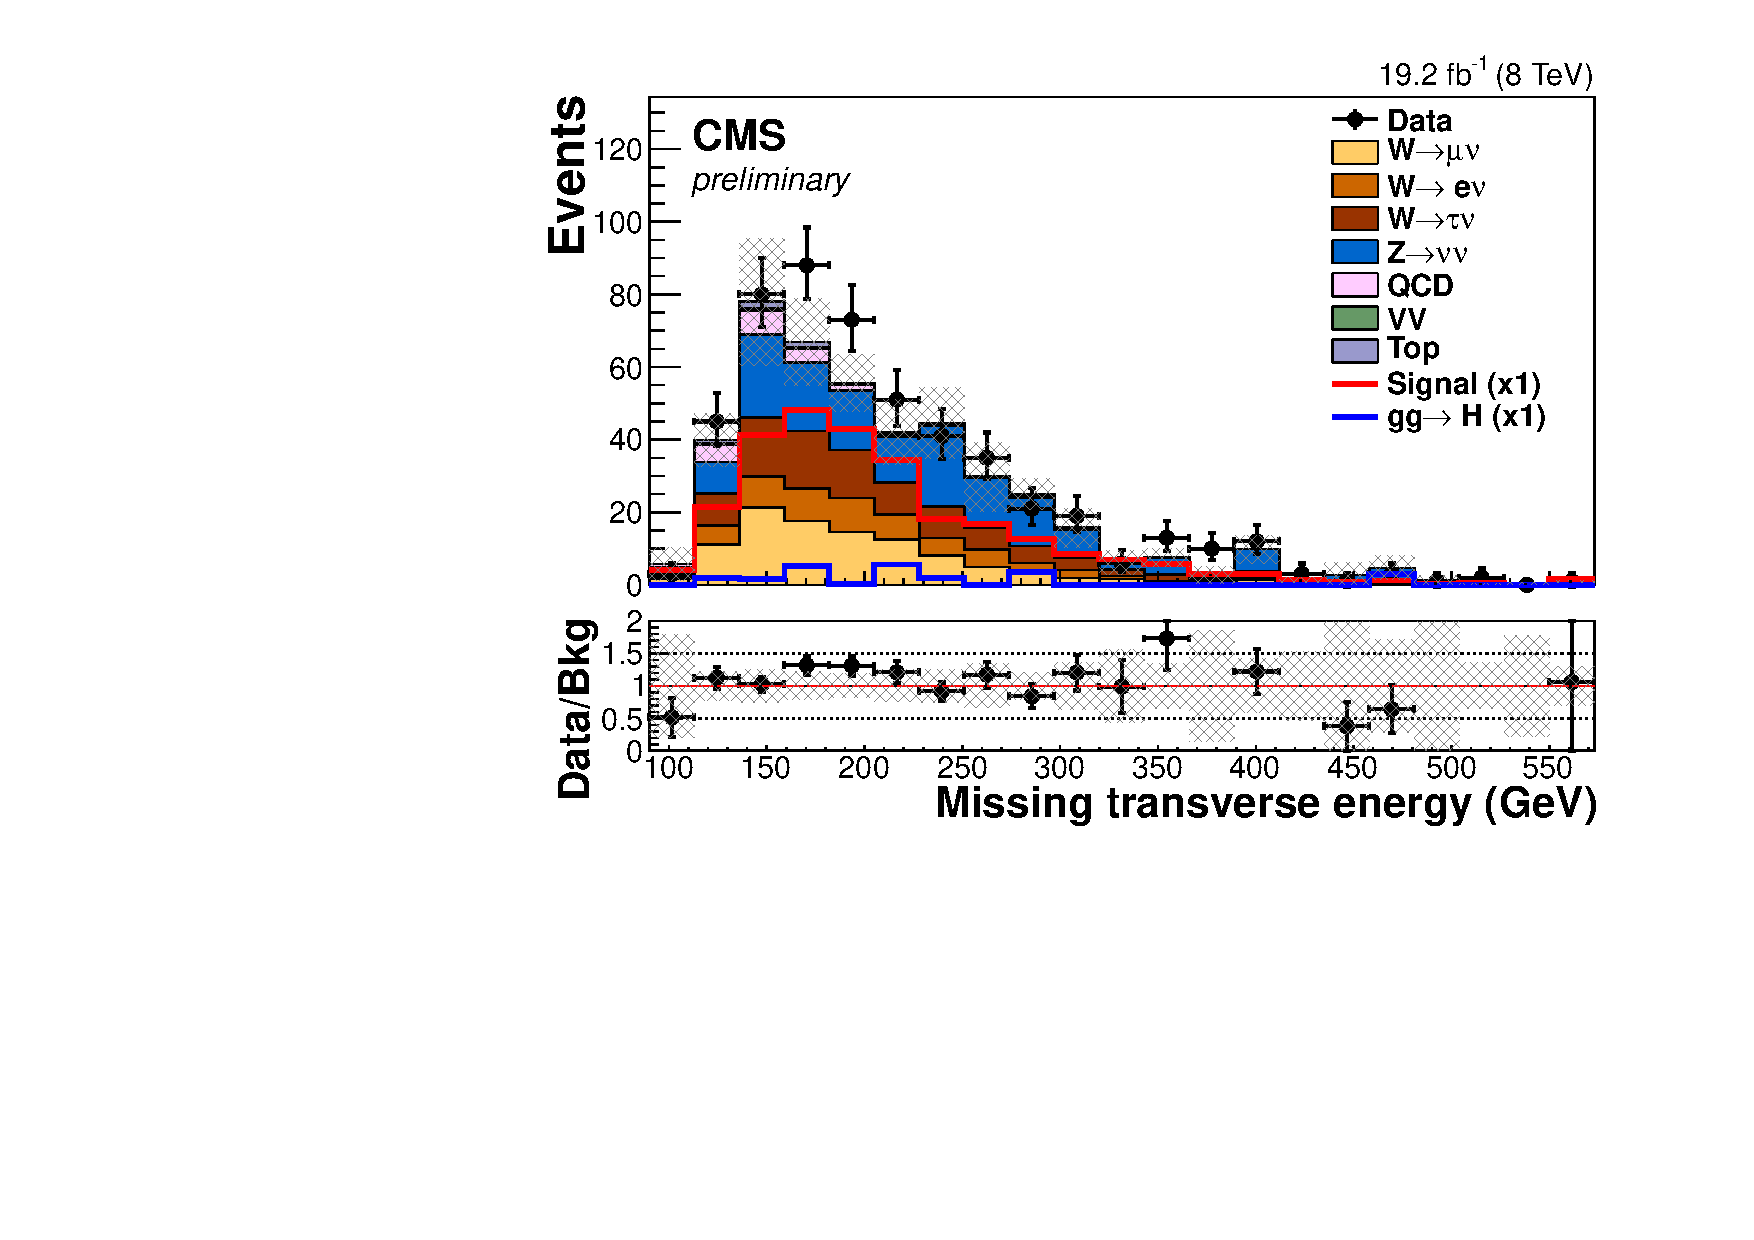
\includegraphics[clip=true,trim=0 0 0 0,width=1.1\textwidth]{../invisible/TalkPics/IOP2015/output_sigreg/nunu_metnomuons.pdf}
      \column{.1\textwidth}
      \hspace{-.5cm}
      \begin{turn}{-90}\scriptsize CMS-PAS-HIG-14-038 \end{turn}
      \end{columns}
    \end{columns}

  \end{frame}

  \begin{frame}
    \frametitle{VBF limits}
          \normalsize
    \begin{columns}
      \column{1.1\textwidth}
            \begin{itemize}
            \item Perform a single bin counting experiment using $CL_{S}$ method
            \item Observed(expected) 95\% C.L. limit on $B(H\rightarrow inv)$ for $m_{H}$=125 GeV is \textcolor{red}{57(40)\%}
            \end{itemize}
    \end{columns}
    \vspace{-0.1cm}
    \begin{columns}
      \column{.03\textwidth}
      \column{.55\textwidth}
      \begin{columns}
        \column{.9\textwidth}
      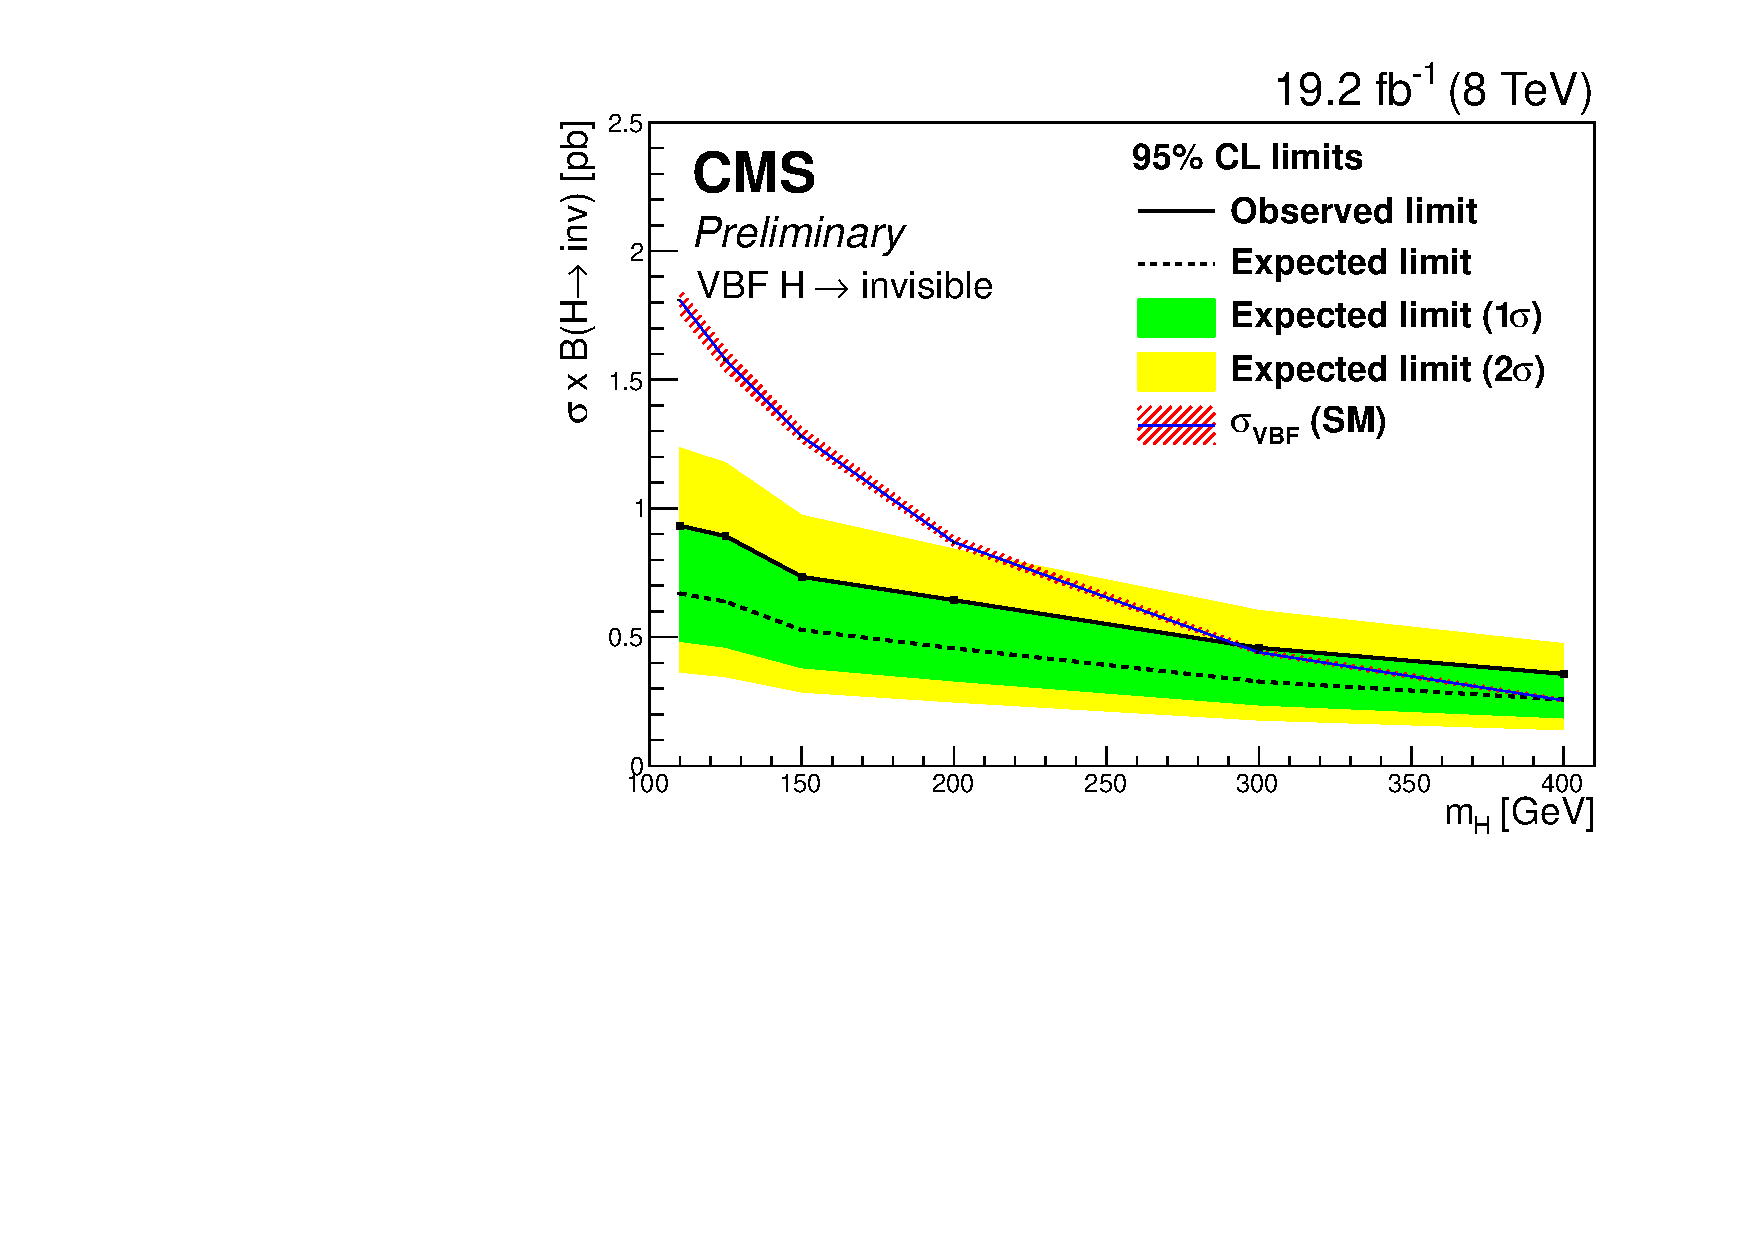
\includegraphics[clip=true,trim=0 0 0 0,width=1.1\textwidth]{../invisible/TalkPics/IOP2015/vbfxslimit.pdf}
      \column{.1\textwidth}
      \hspace{-.5cm}
      \begin{turn}{-90}\scriptsize CMS-PAS-HIG-14-038 \end{turn}
      \end{columns}
      \column{.55\textwidth}
      \begin{columns}
        \column{.9\textwidth}
      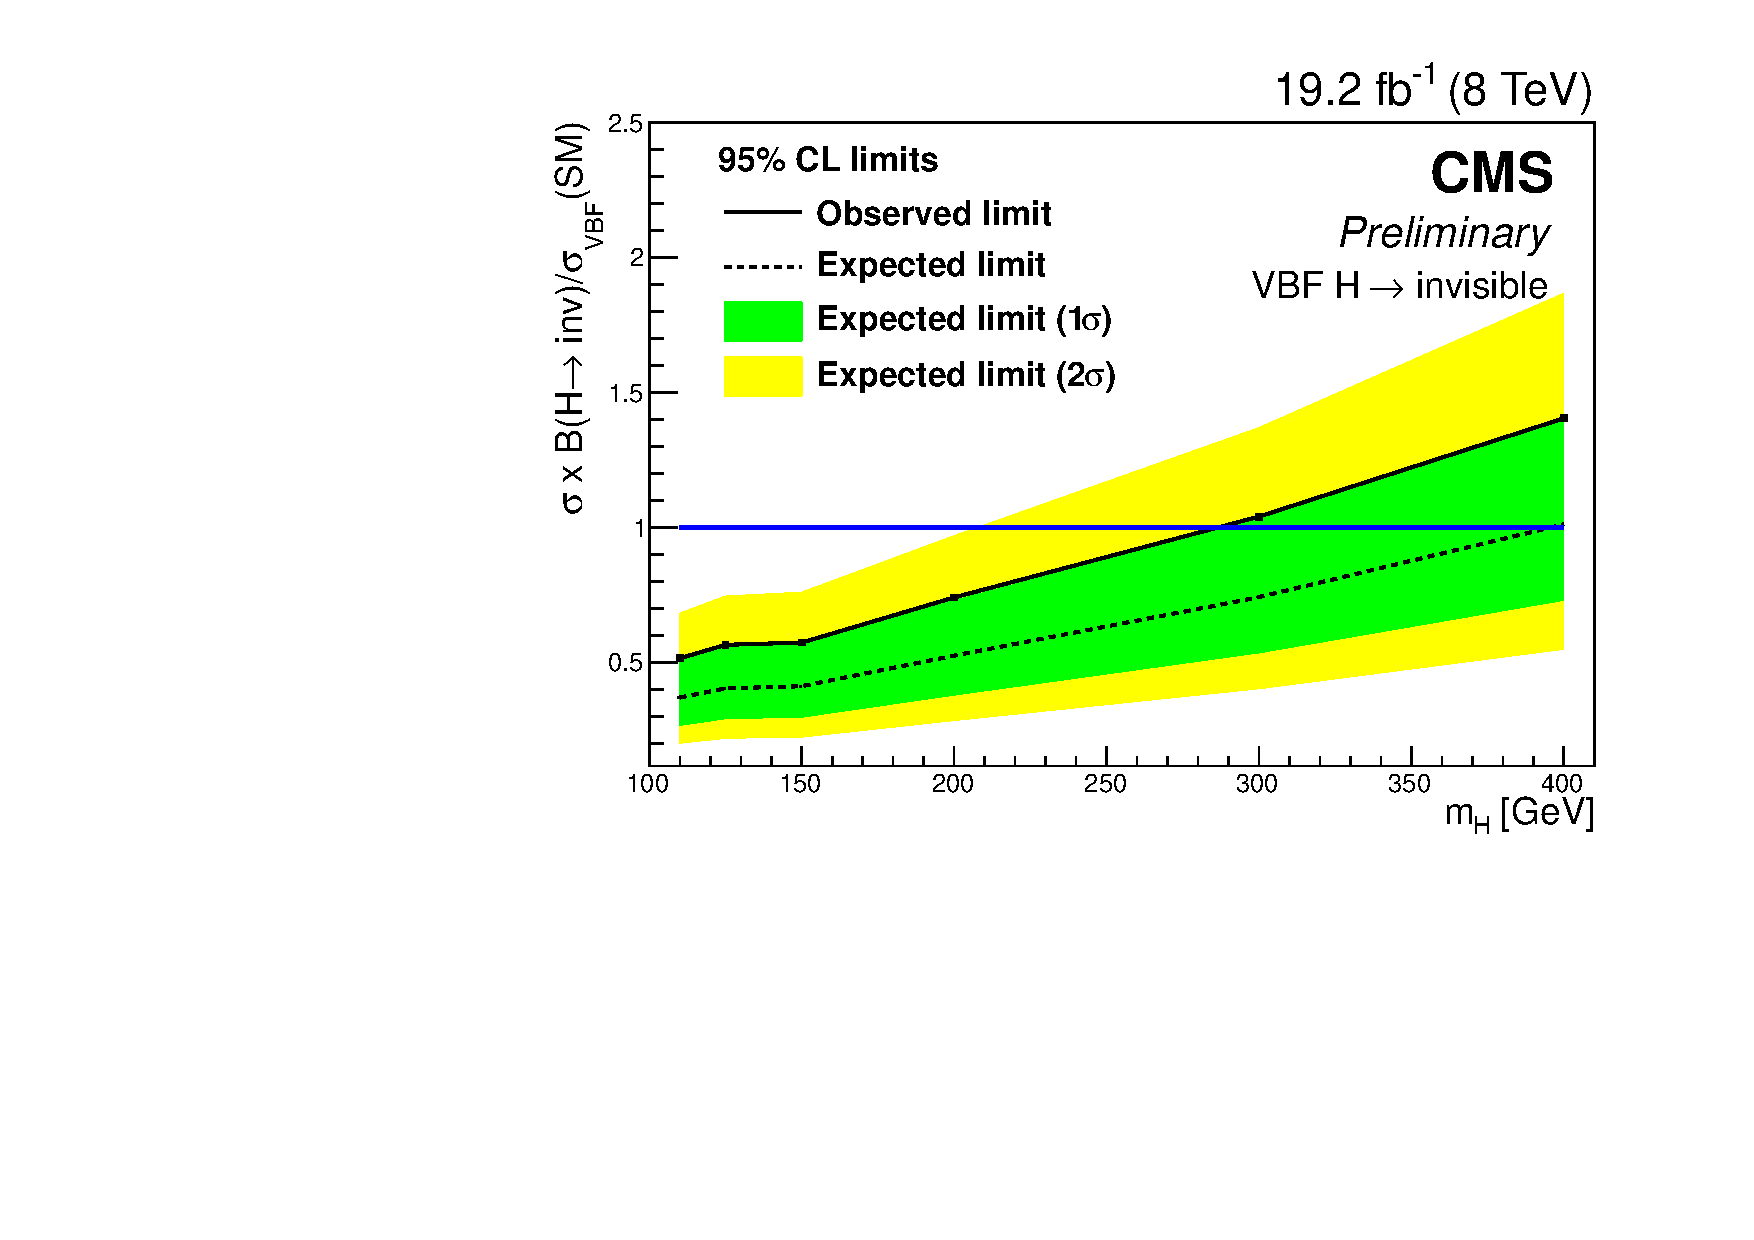
\includegraphics[clip=true,trim=0 0 0 0,width=1.1\textwidth]{../invisible/TalkPics/IOP2015/vbflimit.pdf}
      \column{.1\textwidth}
      \hspace{-.5cm}
      \begin{turn}{-90}\scriptsize CMS-PAS-HIG-14-038 \end{turn}
      \end{columns}
    \end{columns}
  \end{frame}

  \begin{frame}
    \frametitle{Combined Results}
    \begin{itemize}
    \item I was responsible for combining the VBF search results with those in the ZH channels
    \item Separate limits on $\sigma$x$B(H\rightarrow inv)$ are combined at 125 GeV
    \item Assume SM production cross-sections to interpret as a limit on B(H$\rightarrow$inv)
    \end{itemize}
    \begin{columns}
      \column{.5\textwidth}
      Prompt
      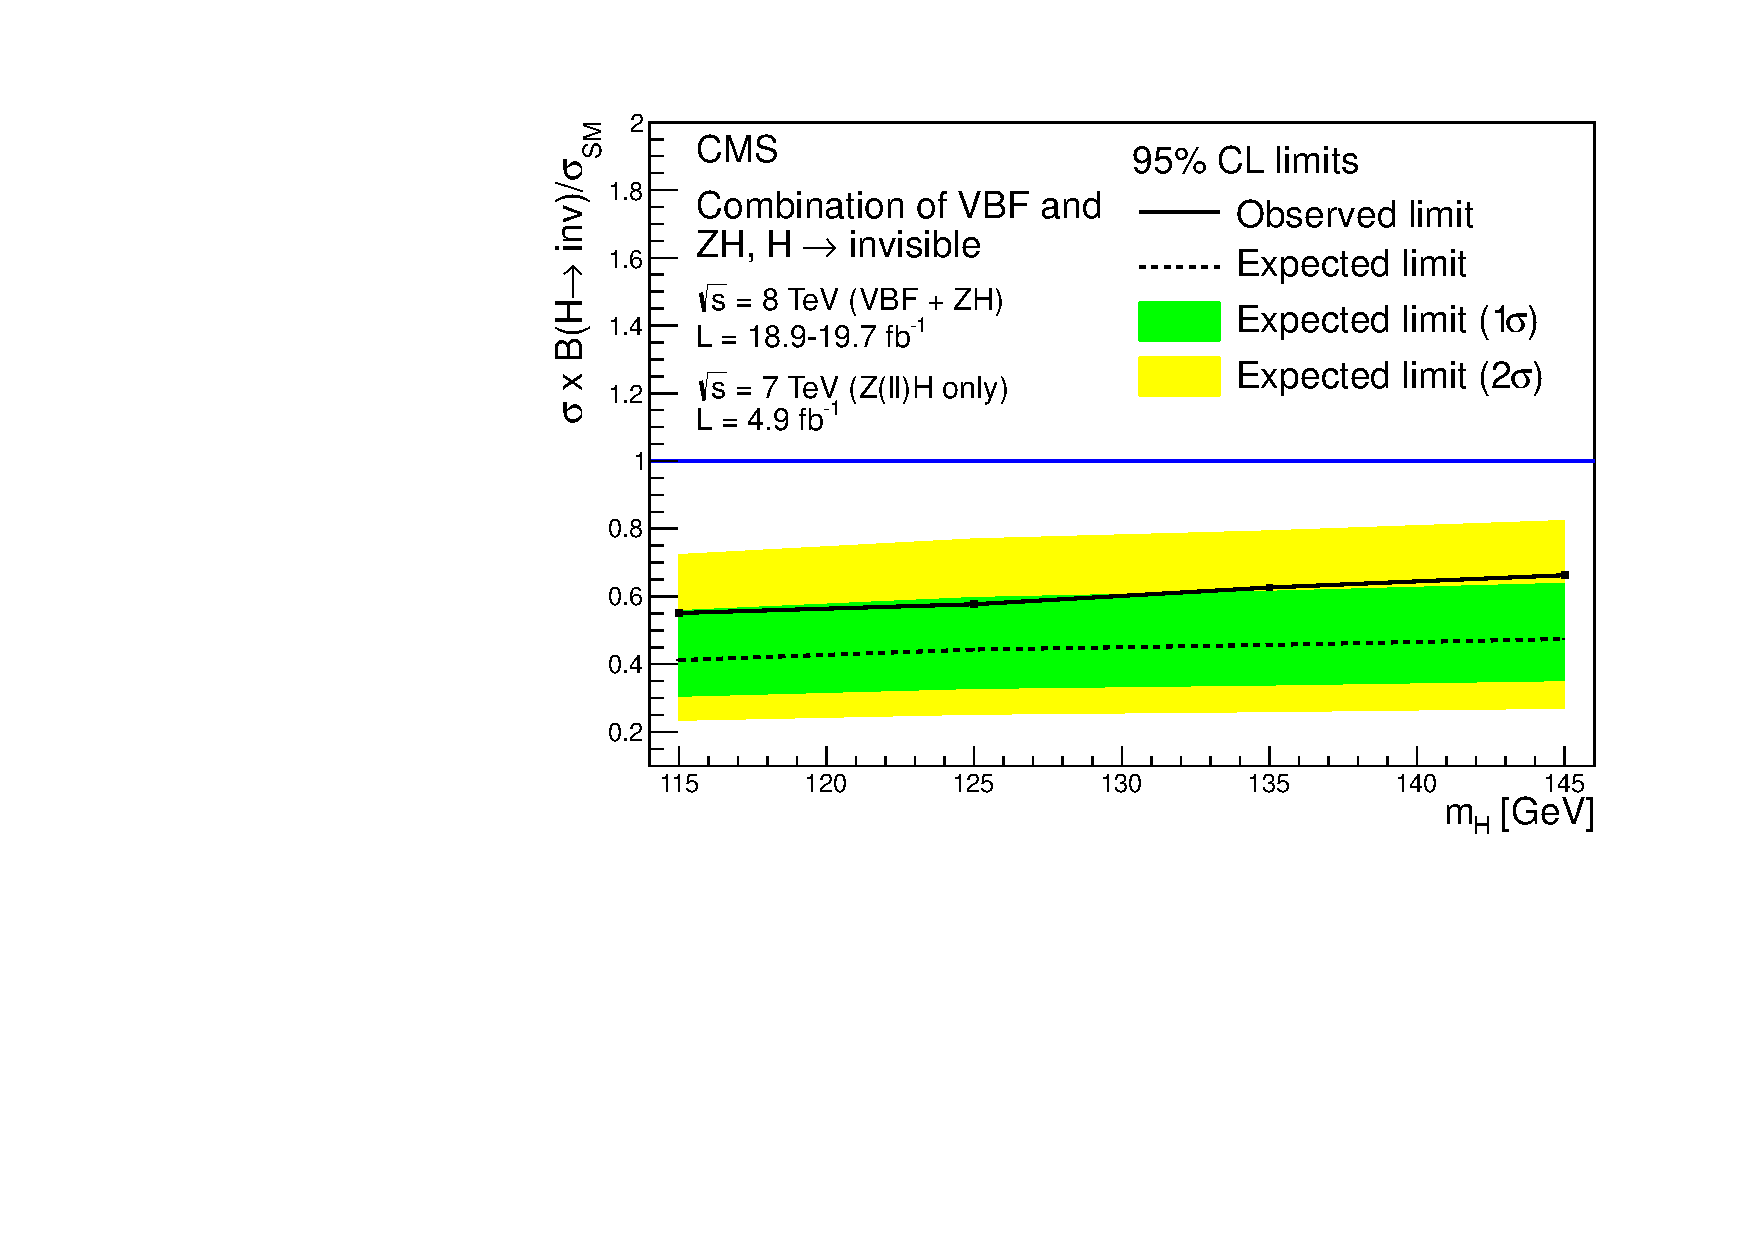
\includegraphics[width=\textwidth]{../invisible/TalkPics/panicpics/combinedlimit.pdf}
      \column{.35\textwidth}
      Parked
      \begin{block}{}
        \footnotesize
        Observed (expected) limits on B(H$\rightarrow$inv) at 95\% C.L. for $m_{H}$=125 GeV

        \centering
        \begin{tabular}{lc}
          \hline
          Channel & Limit/\% \\
          \hline
          VBF & 57(40) \\
          ZH($\ell\ell$+bb) & 81(83) \\
          \hline
          VBF + ZH &{\color{red} 47(35)} \\
          \hline
        \end{tabular}
      \end{block}
    \end{columns}
  \end{frame}




\begin{frame}
  \frametitle{Dark matter interpretations}
    \begin{itemize}
    \item Completed: Parked result has been interpreted in a scalar EFT
    \item In progress: Replicating analysis in Delphes framework for phenomenology paper with other  models
    \end{itemize}
    \centering
    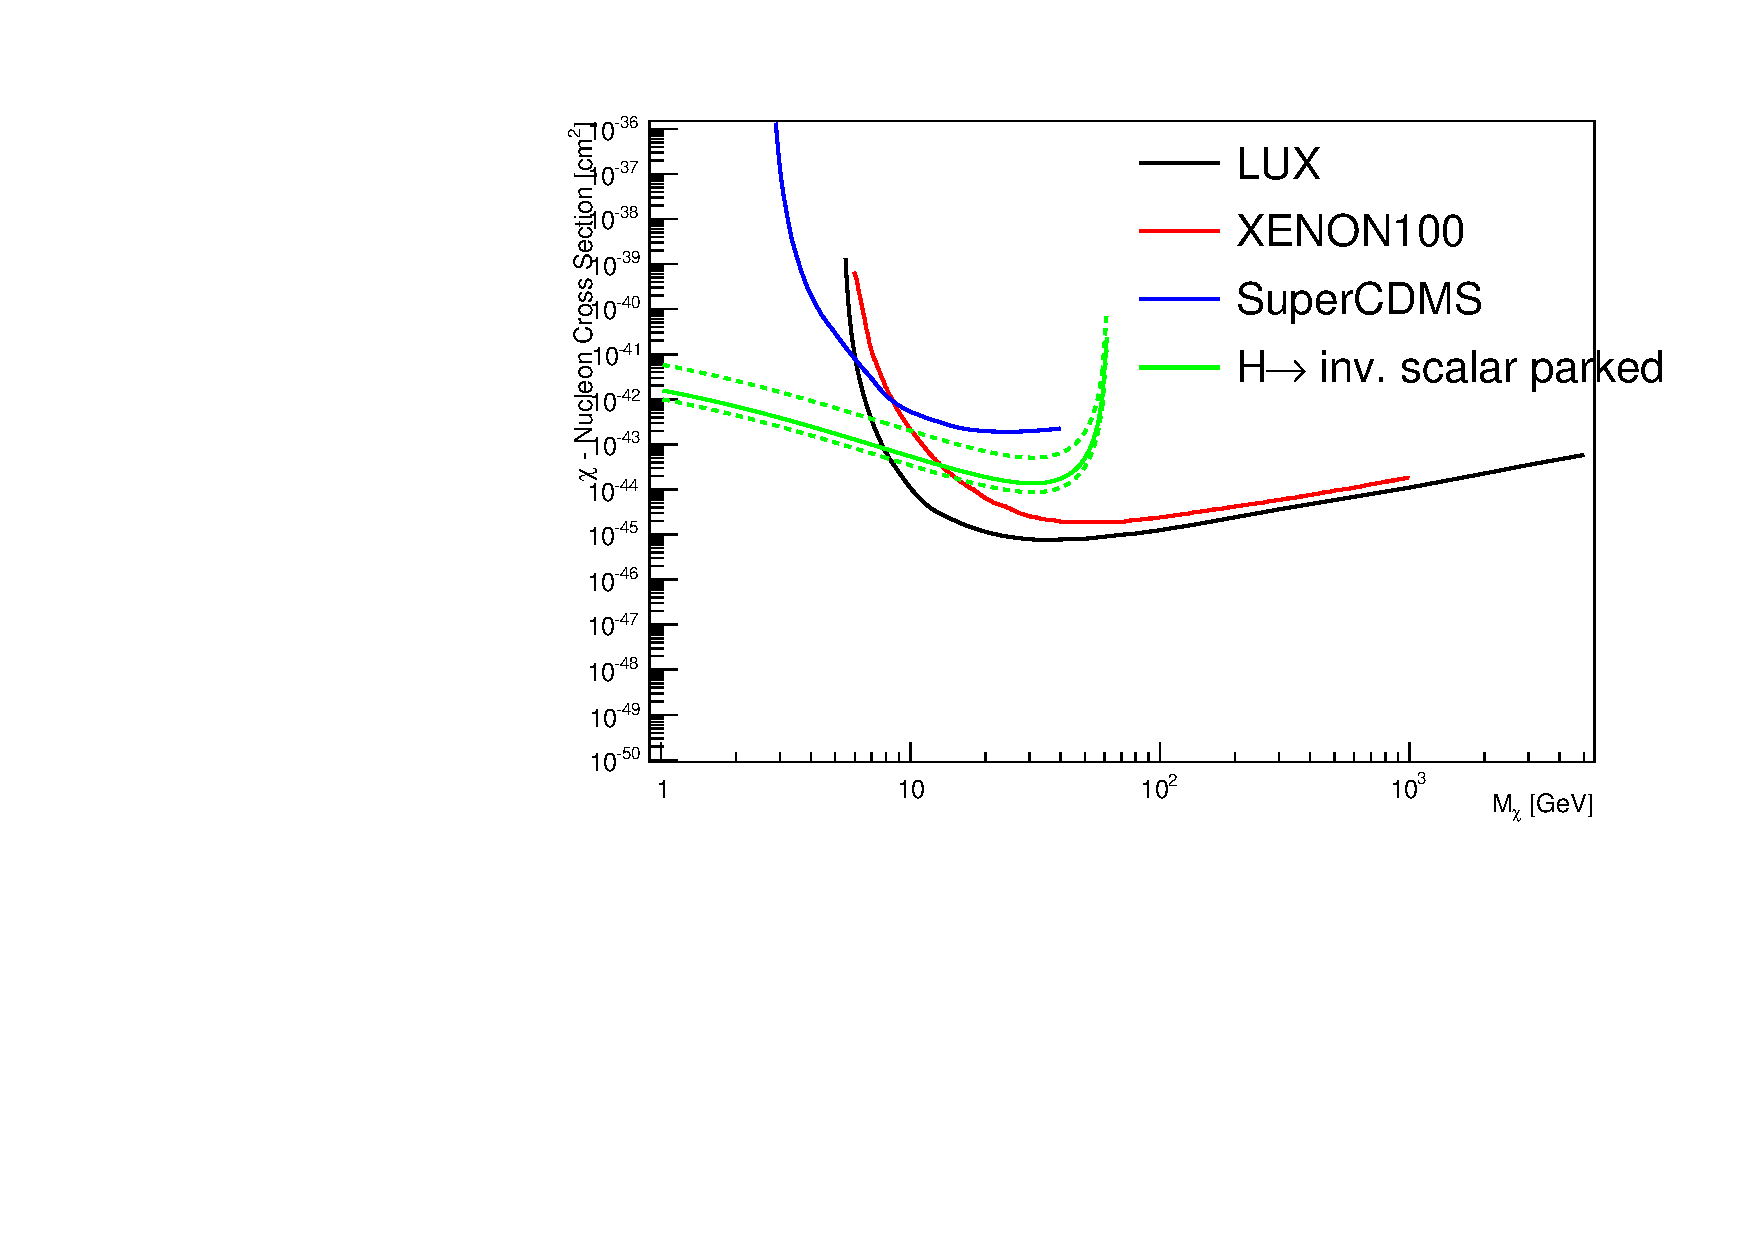
\includegraphics[width=.65\textwidth]{DMplot.pdf}
\end{frame}

\begin{frame}
  \frametitle{Run II}
    \begin{itemize}
    \item Currently working on VBF Higgs to invisible Run II analysis
    \item Contribution to the thesis will depend on progress
    \item Plans:
      \begin{itemize}
      \item Add $\gamma$+jets control region to improve Z estimation
      \item Reoptimise analysis for new kinematics and trigger
      \end{itemize}
    \end{itemize}
\end{frame}

  %% \begin{frame}
  %%   \frametitle{Signatures of Dark Matter (DM)}
  %%   \vspace{-.2cm}
  %%   \begin{columns}
  %%     \column{1.1\textwidth}
  %%   \begin{itemize}
  %%     \item If DM couples to the Higgs the following diagrams are possible
  %%     \end{itemize}
  %%   \vspace{-.2cm}
  %%   \end{columns}
  %%   \begin{columns}
  %%     \column{.35\textwidth}
  %%     \begin{block}{\scriptsize Direct Detection - e.g. LUX}
  %%       \vspace{.3cm}
  %%       \begin{fmfgraph*}(100,70)
  %%         \fmfleft{i1,i2}
  %%         \fmfright{o1,o2}
  %%         \fmf{fermion}{i1,v1,o1}
  %%         \fmf{fermion}{i2,v2,o2}
  %%         \fmf{dashes,label=$H$}{v1,v2}
  %%         \fmffreeze
  %%         \fmflabel{$N$}{i1}
  %%         \fmflabel{$\chi$}{i2}
  %%         \fmflabel{$N$}{o1}
  %%         \fmflabel{$\chi$}{o2}
  %%       \end{fmfgraph*}
  %%       \vspace{.3cm}
  %%     \end{block}

  %%     \column{.35\textwidth}
  %%     \begin{block}{\scriptsize Invisible Higgs - LHC}
  %%       \vspace{.3cm}
  %%       \begin{fmfgraph*}(100,70)
  %%         \fmfleft{i1,i2}
  %%         \fmfright{o1,o2}
  %%         \fmf{fermion}{i1,v1,i2}
  %%         \fmf{fermion}{o1,v2,o2}
  %%         \fmf{dashes,label=$H$}{v1,v2}
  %%         \fmffreeze
  %%         %\fmflabel{$f/w/Z$}{i1}
  %%         \fmflabel{$\chi$}{o1}
  %%         %\fmflabel{$f/W/Z$}{i2}
  %%         \fmflabel{$\chi$}{o2}
  %%       \end{fmfgraph*}
  %%       \vspace{.3cm}
  %%     \end{block}
  %%     \column{.35\textwidth}
  %%     \begin{block}{\scriptsize Annihilation - e.g. WMAP}
  %%       \vspace{.3cm}
  %%       \begin{fmfgraph*}(100,70)
  %%         \fmfleft{i1,i2}
  %%         \fmfright{o1,o2}
  %%         \fmf{fermion}{i1,v1,i2}
  %%         \fmf{fermion}{o1,v2,o2}
  %%         \fmf{dashes,label=$H$}{v1,v2}
  %%         \fmffreeze
  %%         %\fmflabel{$f/w/Z$}{i1}
  %%         \fmflabel{$\chi$}{i1}
  %%         %\fmflabel{$f/W/Z$}{i2}
  %%         \fmflabel{$\chi$}{i2}
  %%       \end{fmfgraph*}
  %%       \vspace{.3cm}
  %%     \end{block}
  %%   \end{columns}
  %%   \begin{columns}
  %%     \column{1.1\textwidth}
  %%     \begin{itemize}
  %%     \item Limits on $\mathcal{B}$(H$\rightarrow$inv) complement/are complemented by other experiments
  %%     \end{itemize}
  %%   \end{columns}
  %% \end{frame}

%!!FOCUS MORE ON VBF AND CHANGE TO HOW TO DETECT INVISIBLE AT CMS
  \begin{frame}%!!REVISIT AT END
    \frametitle{Conclusions}
    \label{lastframe}
    \begin{itemize}
    \item The thesis will focus on the parked data VBF Higgs to invisible analysis
    \item The majority of work is complete
    \item Items still in progress are:
      \begin{itemize}
      \item Further work on interpretations
      \item[-] Aiming for a phenomenology paper by end of year
      \item Run II
      \item[-] Dependent on progress
      \end{itemize}
    \item On track to submit before funding runs out in March 2016
    \end{itemize}
    


  \end{frame}

  \begin{frame}
    \frametitle{Backup}
  \end{frame}

  \begin{frame}
    \frametitle{ZH: summary}
    \begin{columns}
      \column{1.1\textwidth}
    \begin{itemize}
    \item Search also performed in $ZH\rightarrow\ell\ell inv$ and $ZH\rightarrow b\bar{b} inv$ channels at CMS
    \item Observed(expected) 95\% C.L. limit on $B(H\rightarrow inv)$ for $m_{H}$=125 GeV is \textcolor{red}{81(83)\%}
      \begin{columns}
        \column{.55\textwidth}
      \begin{columns}
        \column{.9\textwidth}
      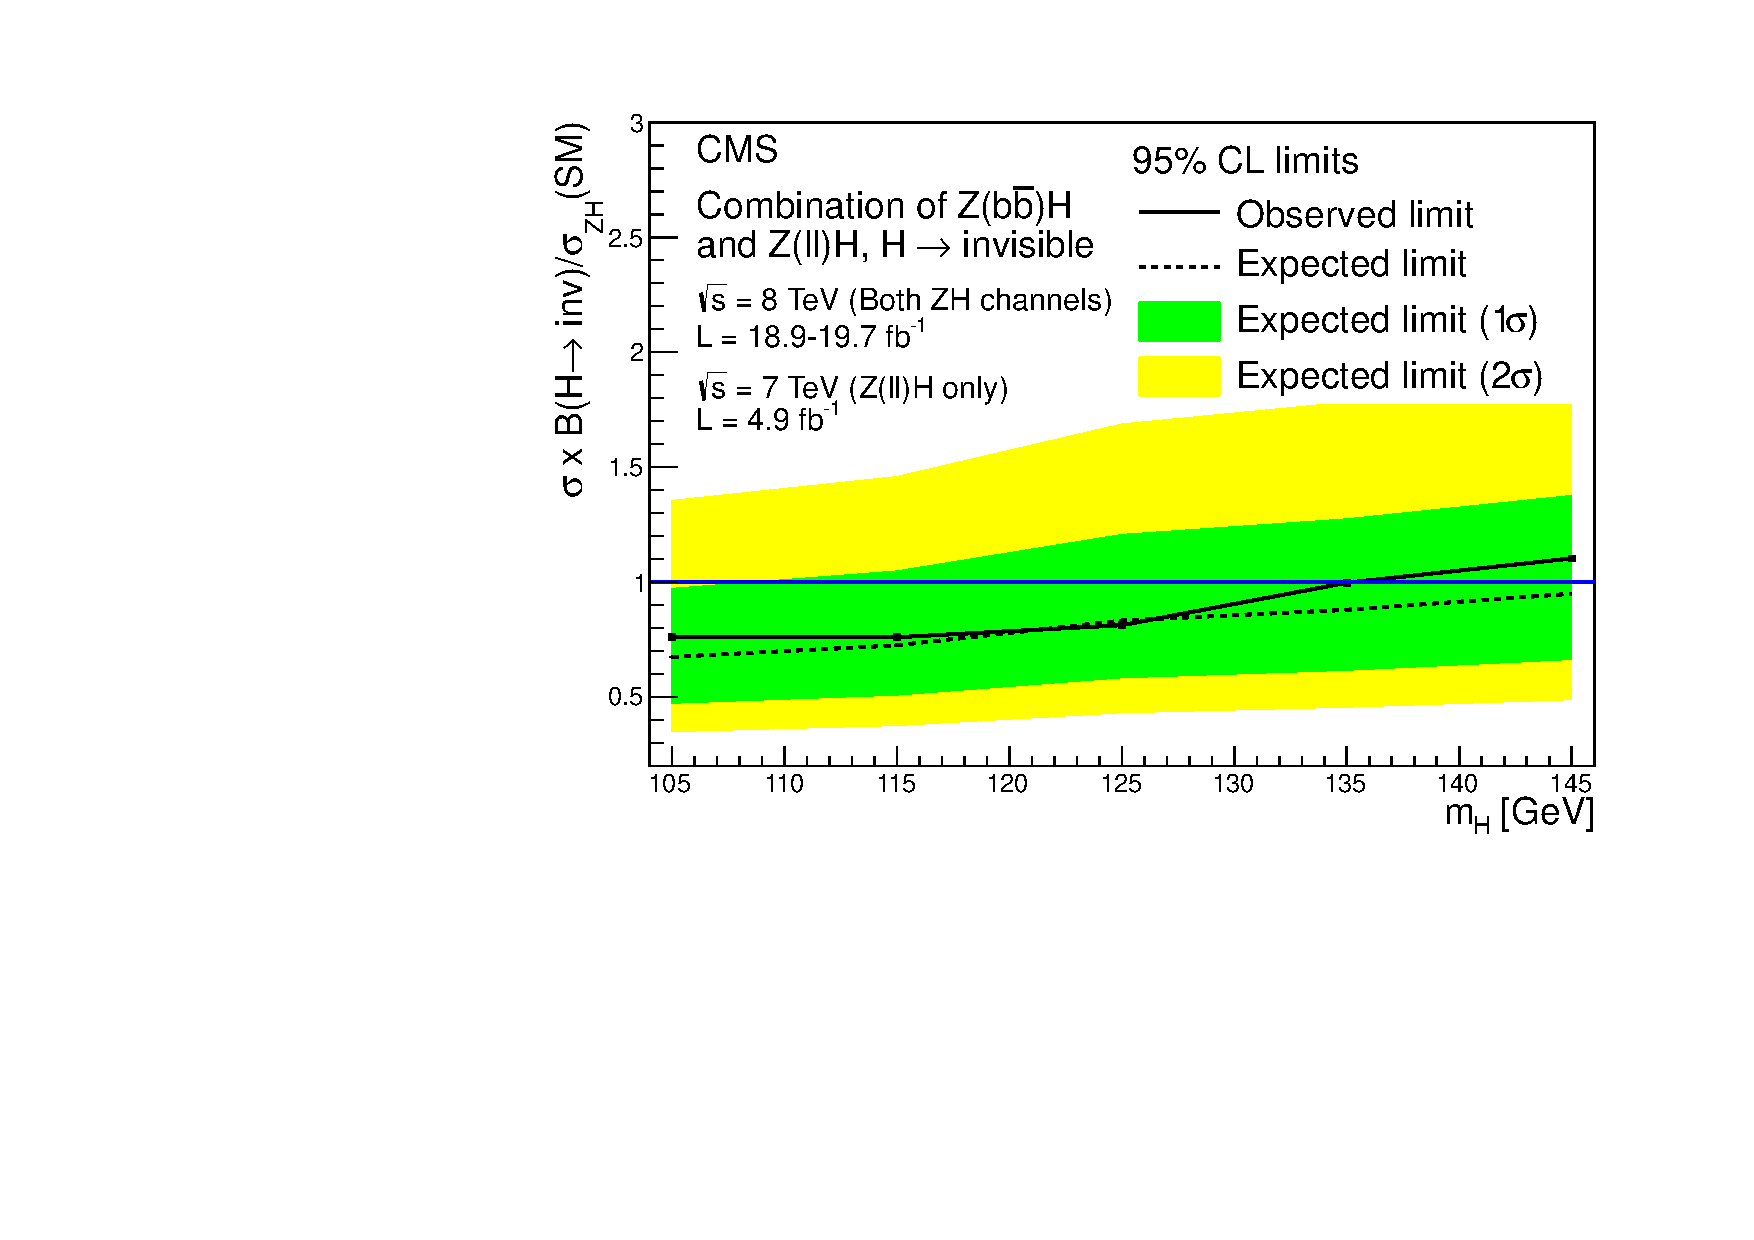
\includegraphics[clip=true,trim=0 0 0 0,width=1.1\textwidth]{../invisible/TalkPics/panicpics/zhlimit.pdf}
      \column{.1\textwidth}
      \hspace{-.5cm}
      \begin{turn}{-90}\scriptsize Eur. Phys. J. C 74 (2014) 2980 \end{turn}
      \end{columns}
      \end{columns}
      \end{itemize}
    \end{columns}
  \end{frame}



  \begin{frame}%!!MAKE SURE OK
    \frametitle{References}
      \begin{itemize}
      \item CMS Higgs combination - CMS--HIG-14-009
      \item CMS VBF Higgs to invisible parked data PAS - CMS-PAS-HIG-14-038
      \item CMS Higgs to invisible paper - Eur. Phys. J. C 74 (2014) 2980
      \end{itemize}
  \end{frame}

  %!!
  \begin{frame}
    \frametitle{Comparison to recent ATLAS result}
    \begin{itemize}
    \item We see an excess where ATLAS see a deficit:
    \item[-] observed can move the post-fit expected limit
    \item[-] were we to see a similar deficit our expected limit improves by $\sim$10\%
    \item ATLAS use a single data driven normalisation factor for all V+jets backgrounds
    \item[-] statistical uncertainty on the factor is therefore lower
    \item[-] reducing our $Z\rightarrow\nu\nu$ statistical uncertainty to the level we see in $W\rightarrow\mu\nu$ our expected limit improves by $\sim$10\%
    \end{itemize}
  \end{frame}

  %!!
  \begin{frame}
    \frametitle{W+jets}
    \begin{itemize} 
    \item $W\rightarrow e/\mu\nu$ control region formed by swapping lepton veto for $e/\mu$ requirement
    \item $W\rightarrow \tau\nu$ control region formed by requiring a hadronic tau
    \item[-] not many events with hadronic taus, need to loosen requirements
    \item[-] assign a 20\% systematic to $W\rightarrow\tau\nu$ to compensate
   \end{itemize}
    \begin{block}{}
      \centering
      $N_{bkg}^{sig}=(N_{obs}^{control}-N_{other\,bkgs}^{control})\cdot \frac{N_{MC}^{sig}}{N_{MC}^{control}}$
      \begin{tabular}{|l|c|}
        \hline
        $W\rightarrow\mu\nu$&$102.5 \pm 6.2 \pm 11.7$\\
$W\rightarrow e\nu$&$57.9 \pm 7.4 \pm 7.7$\\
$W\rightarrow\tau\nu$&$94.6 \pm 13.1 \pm 23.8$\\
        \hline
      \end{tabular}
    \end{block}
  \end{frame}

  %!!
  \begin{frame}
    \frametitle{Z+jets}
    \begin{itemize}
    \item Use $Z\rightarrow\mu\mu$ MC ignoring muons to emulate $Z\rightarrow\nu\nu$
    \item Correct for difference in cross-section
    \item Efficiency correction takes into account EWK vs QCD difference
    \end{itemize}
    \begin{block}{}
      \centering
      $N_{S}^{Z\rightarrow\nu\nu}=\left(N_{C}^{Data}-N_{C}^{bkg}\right) \cdot\frac{\sigma\left(Z\rightarrow\nu\nu\right)}{\sigma\left(Z\rightarrow\mu\mu\right)}\cdot \frac{\epsilon_{S}^{ZMC}}{\epsilon_{C}^{ZMC}}$
      \begin{tabular}{|l|c|}
        \hline
        $Z\rightarrow\nu\nu$&$158.1 \pm 37.3 \pm 21.2$\\
        \hline
      \end{tabular}
    \end{block}
  \end{frame}

  %!!
  \begin{frame}
    \frametitle{}
      \begin{block}{QCD}
        \begin{itemize}       
      \item Take shape from region with third jet near MET
      \item Normalise in sideband region
      \item[-] normalisation highly selection dependent
      \item[-] parameterise as function of selection and extrapolate
      \item Final estimate $17\pm 14$\\
    \end{itemize}
    \end{block}
    \begin{block}{Other backgrounds}
      \begin{itemize}
      \item Taken from MC
      \end{itemize}
      \centering
      \begin{tabular}{|l|c|}
        \hline
        top & $5.5 \pm  1.8$\\
        VV & $3.9 \pm 0.7$\\
        \hline
        \end{tabular}
    \end{block}

  \end{frame}

  \begin{frame}
    \frametitle{Z($\ell\ell$)H outline}
    \begin{columns}
      \column{.56\textwidth}
      \vspace{-.5cm}
      \begin{block}{\scriptsize Signal Topology and Selection}
        \scriptsize
        \begin{itemize}
        \item Two same flavour opposite sign electrons or muons
          \ssmall
        \item[-] $p_{T}>20$ GeV, $|M_{\ell\ell}-m_{Z}|<15$ GeV
          \scriptsize
        \item Large MET
          \ssmall
        \item[-] $MET>120$ GeV
        \end{itemize}
      \end{block}
      \begin{block}{\scriptsize Backgrounds and Rejection Cuts}
        \scriptsize
        \begin{itemize}
        \item ZZ($\ell\ell\nu\nu$)+jets, WW($\ell\nu\ell\nu$)+jets
        \item WZ($\ell\nu\ell\ell$)+jets
          \ssmall
        \item[-] Veto events with $>$3 leptons, $p_{T}$$>$10 GeV
          \scriptsize
        \item Z($\ell\ell$)+jets
          \ssmall
        \item[-] MET cut, MET-$\ell\ell$ balance requirement
          \scriptsize
        \item $t\bar{t}$, single top, W($\ell\nu$), QCD
          \ssmall
        \item[-] $\leq$1 jet, $p_{T}$$>$30 GeV
        \item[-] no b-tagged jets, $p_{T}>30$ GeV
        \end{itemize}
      \end{block}
      \column{.44\textwidth}
      \centering
      \begin{fmfgraph*}(75,40)
        \fmfleft{i1,i2}
        \fmfright{o1,o2,o3}
        \fmf{fermion}{i1,v1,i2}
        \fmf{photon,label=$Z$}{v1,v2}
        \fmf{photon}{v2,v4}
        \fmf{photon,label=$Z$,l.side=right}{v4,v3}
        \fmf{fermion}{o1,v3,o2}
%        \fmf{photon}{v5,v3}
        \fmf{dashes,label=$H$,l.side=left}{v2,o3}
        \fmflabel{$\ell^{+}$}{o1}
        \fmflabel{$\ell^{-}$}{o2}
        \fmflabel{$q$}{i1}
        \fmflabel{$\bar{q}$}{i2}
      \end{fmfgraph*}
      \vspace{.4cm}
      \begin{columns}
        \column{.05\textwidth}
        \column{.9\textwidth}
        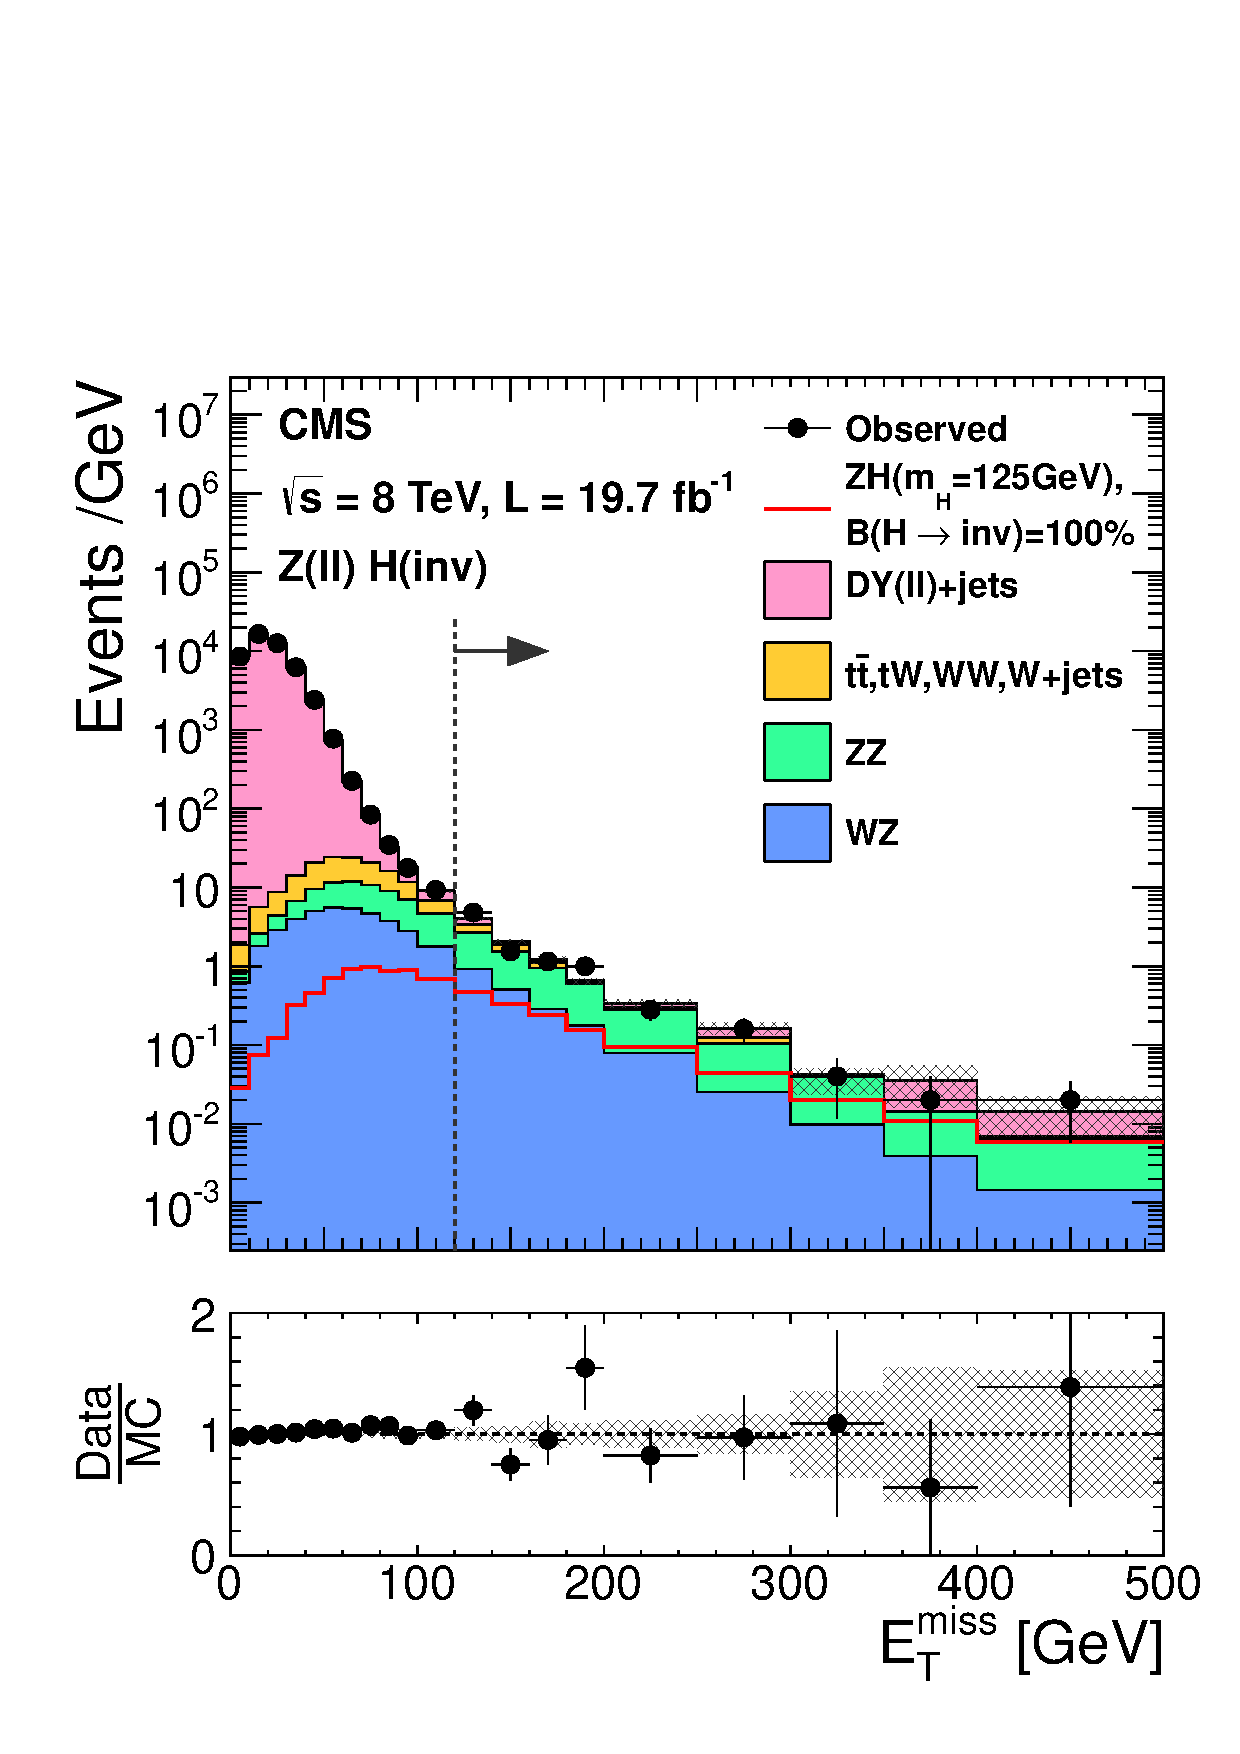
\includegraphics[clip=true,trim=0 0 0 20, width=\textwidth]{../invisible/TalkPics/panicpics/zllmet.pdf}
        \column{.1\textwidth}
        \hspace{-.4cm}\begin{turn}{-90}\scriptsize arXiv:1404.1344 \end{turn}
      \end{columns}
    \end{columns}

  \end{frame}
  \begin{frame}
    \frametitle{ Z($\ell\ell$)H background estimation}
    \vspace{-.25cm}
    \begin{columns}
      \column{1.06\textwidth}
    \begin{block}{\scriptsize ZZ($\ell\ell\nu\nu$)+jets and WZ($\ell\nu\ell\ell$+jets)}
      \scriptsize
      \begin{itemize}
      \item Estimated from MC prediction
      \end{itemize}
    \end{block}
    \end{columns}
    \vspace{.2cm}
    \begin{columns}
      \column{.5\textwidth}
    \begin{block}{\scriptsize Z($\ell\ell$)+jets}
      \scriptsize
      \begin{itemize}
      \item Estimated from photon + jets events
      \item[-] Photon $p_{T}$ spectrum reweighted to match Z spectrum
      \end{itemize}
    \end{block}
      \column{.5\textwidth}
      \begin{columns}
        \column{.5\textwidth}
        \centering
      \begin{fmfgraph*}(50,40)
        \fmfleft{i1,i2}
        \fmfright{o1,o2,o3}
        \fmf{gluon}{i2,v1}
        \fmf{fermion}{i1,v1,v2,o3}
        \fmf{photon}{v2,v4}
        \fmf{photon,label=$Z$,l.side=right}{v4,v5}
        \fmf{fermion}{o1,v5,o2}
        \fmflabel{$q$}{i1}
        \fmflabel{$q$}{o3}
        \fmflabel{$g$}{i2}
        \fmflabel{$\ell^{-}$}{o2}
        \fmflabel{$\ell^{+}$}{o1}
      \end{fmfgraph*}
      \column{.5\textwidth}
      \centering
      \begin{fmfgraph*}(50,40)
        \fmfleft{i1,i2}
        \fmfright{o1,o2}
        \fmf{gluon}{i2,v1}
        \fmf{fermion}{i1,v1,v2,o2}
        \fmf{photon}{v2,v4}
        \fmf{photon}{v4,o1}
        \fmflabel{$q$}{i1}
        \fmflabel{$q$}{o2}
        \fmflabel{$g$}{i2}
        \fmflabel{$\gamma$}{o1}
      \end{fmfgraph*}
      \end{columns}
    \end{columns}
    \begin{columns}
      \column{1.06\textwidth}
    \begin{block}{\scriptsize WW($\ell\nu\ell\nu$)+jets, single top, $t\bar{t}$, $Z(\tau\tau$)}
      \scriptsize
      \begin{itemize}
      \item Estimated from $e\mu$ events and Z peak sidebands:
        \ssmall
        \vspace{-.1cm}
      \item[-] $m_{\ell\ell}$ 40-70 and 110-200 GeV
        \scriptsize
      \item[-] $N_{\ell\ell}^{sig}=N^{sig}_{e\mu}\cdot N_{\ell\ell}^{SB}/N_{e\mu}^{SB}$

      \end{itemize}
    \end{block}
    \end{columns}
  \end{frame}

  \begin{frame}
    \frametitle{Z($\ell\ell$)H results}
    \vspace{-.2cm}
      \vspace{-.2cm}
    \begin{block}{}
      \tiny
      \centering
      \begin{tabular}{cccccc}
        \hline
        \vspace{-.05cm}
        & Process & \multicolumn{2}{c}{$\sqrt{s}=7$TeV} & \multicolumn{2}{c}{$\sqrt{s}=8$TeV} \\
        \vspace{-.05cm}
        & & ee & $\mu\mu$ & ee & $\mu\mu$ \\
        \hline
        \vspace{-.05cm}
        0 jets & Total backgrounds & $8.7\pm 6.5$ & $11.0\pm 3.3$ & $37.4\pm 3.7$ & $51.6\pm 4.8$ \\
        & ZH(125) & $2.3\pm 0.2$ & $3.1\pm 0.3$ & $10.3\pm 1.2$ & $14.7\pm 1.5$ \\
        & Observed data & 9 & 10 & 36 & 46 \\
        \hline
        & S/B for B(H$\rightarrow$inv) 100\% & 0.26 & 0.28 & 0.28 & 0.24 \\ 
        \hline
        1 jet & Total backgrounds & $2.6\pm 0.7$ & $2.8\pm 0.9$ & $10.6\pm 4.2$ & $13.8\pm 5.8$ \\
        & ZH(125) & $0.4\pm 0.1$ & $0.5\pm 0.1$ & $1.6\pm 0.2$ & $2.5\pm 0.3$ \\
        & Observed data & 1 & 4 & 11 & 17  \\
        \hline
        & S/B for B(H$\rightarrow$inv) 100\% & 0.15  & 0.18 & 0.15 & 0.18 \\ 
        \hline
      \end{tabular}
      \end{block}
    \vspace{-.4cm}
    \begin{columns}
      \column{.4\textwidth}
      \column{.3\textwidth}
    \scriptsize arXiv:1404.1344
    \vspace{-.2cm}
      \column{.3\textwidth}
    \scriptsize arXiv:1404.1344
    \vspace{-.2cm}
    \end{columns}
    \begin{columns}
      \column{1.05\textwidth}
    \begin{columns}
     \column{.4\textwidth}
     \hspace{.1cm}
     \begin{block}{}
       \scriptsize
       \begin{itemize}
       \item Limits obtained from a 2D fit to $m_{T}$ and $\Delta\phi (\ell\ell)$
       \item[-] 1D fit to $m_{T}$ for 7 TeV data
       \item Assuming SM Higgs production cross-section and acceptance:
       \item[-]  observed(expected) 95\% C.L. limit on $B(H\rightarrow inv)$ for $m_{H}$=125 GeV is 83(86)\%
       \end{itemize}

    \end{block}
     \column{.29\textwidth}
     \begin{columns}

       \column{.95\textwidth}
       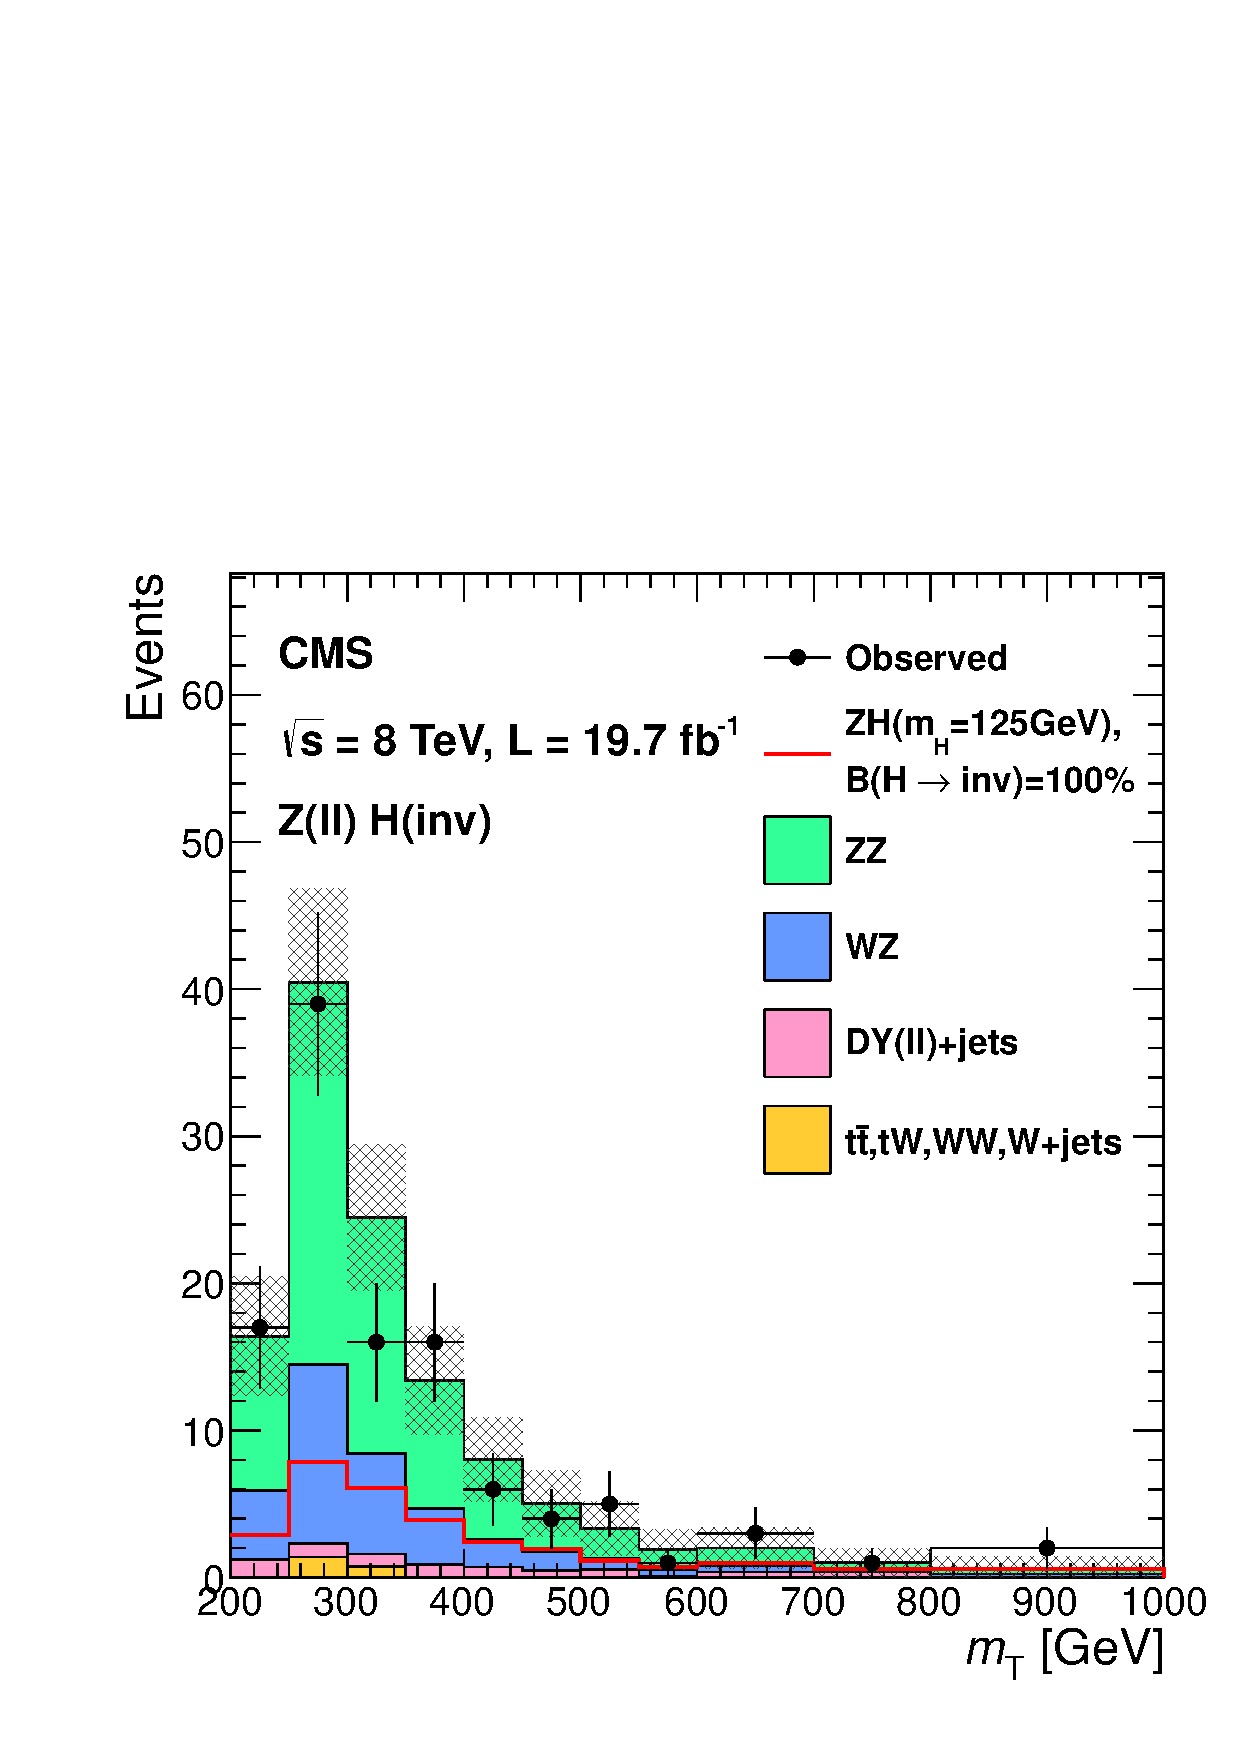
\includegraphics[clip=true,trim=25 0 0 20, height=.53\textheight]{../invisible/TalkPics/panicpics/zllmt.pdf}
       \column{.06\textwidth}

     \end{columns}
    \column{.29\textwidth}
     \begin{columns}
       \column{.95\textwidth}
       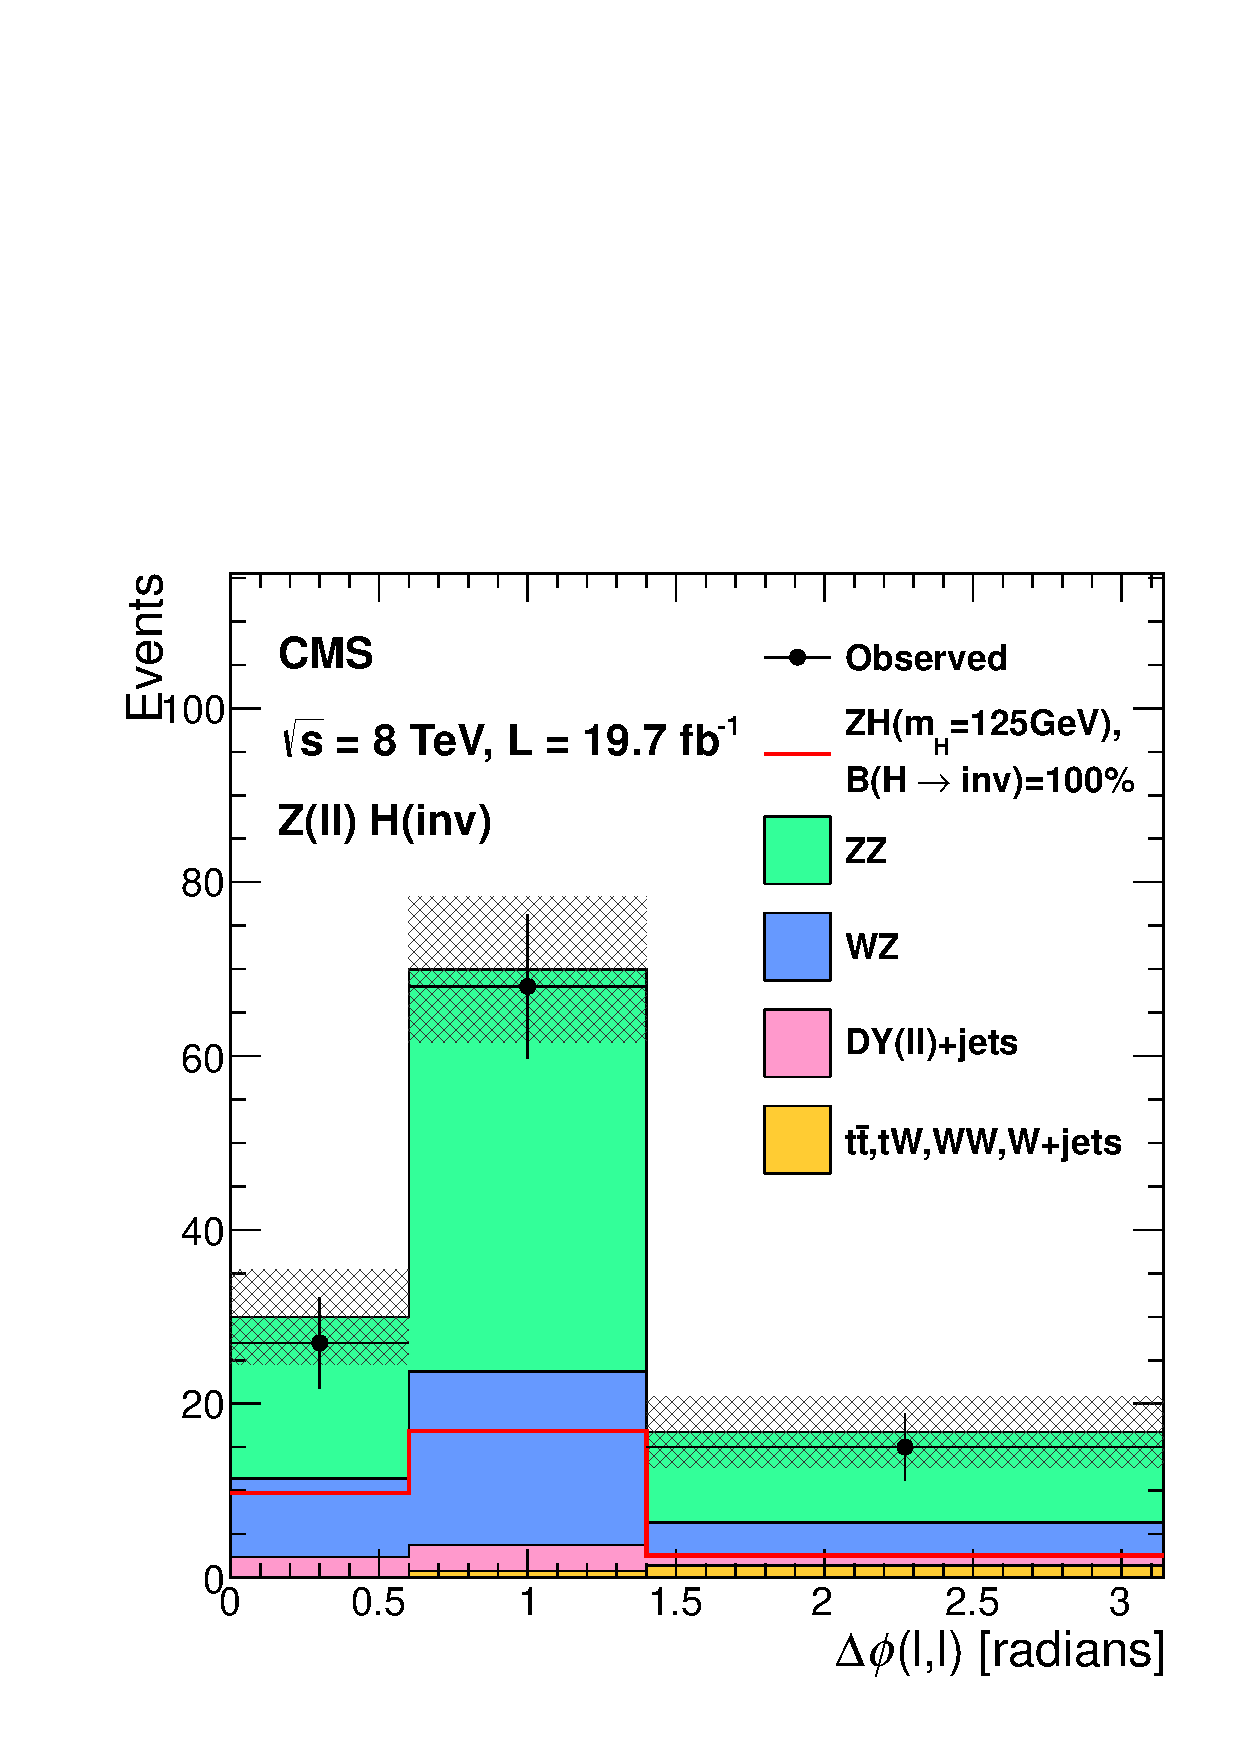
\includegraphics[clip=true,trim=25 0 0 20, height=.53\textheight]{../invisible/TalkPics/panicpics/zlldphi.pdf}
       \column{.05\textwidth}
     \end{columns}


    \end{columns}
    \end{columns}
  \end{frame}


  \begin{frame}
    \frametitle{Z(bb)H outline and backgrounds}
    \vspace{.4cm}
    \begin{columns}
      \column{.56\textwidth}
      \vspace{-.82cm}
      \begin{block}{\scriptsize Signal Topology and Selection}
        \scriptsize
        \begin{itemize}
          \vspace{-.05cm}
        \item Two b-tagged jets:
          \vspace{-.05cm} 
         \ssmall
        \item[-]$p_{T}>30/60$ GeV, $p_{Tjj}>100-130$ GeV
            \scriptsize
        \item Three bins in MET
          \vspace{-.05cm}
          \ssmall
        \item[-] 100-130, 130-170, $>170$ GeV
                  \end{itemize}
      \end{block}
      \vspace{-.15cm}
      \begin{block}{\scriptsize Backgrounds and Rejection Cuts}
        \scriptsize
        \begin{itemize}
          \vspace{-.05cm}
        \item Z($\nu\nu$)+jets, W($\ell\nu$)+jets
          \vspace{-.05cm}
        \item ZZ($\nu\nu b\bar{b}$)
          \vspace{-.05cm}
        \item WZ($\ell\nu b\bar{b}$), $t\bar{t}$, single top
          \vspace{-.05cm}
          \ssmall
        \item[-] Veto events with leptons, $p_{T}$$>$15 GeV
          \scriptsize
          \vspace{-.05cm}
        \item QCD
          \vspace{-.05cm}
          \ssmall
        \item[-] MET quality requirements
          \vspace{-.05cm}
        \end{itemize}
      \end{block}
      \vspace{-.15cm}
      \begin{block}{\scriptsize Background estimation - data normalised MC}
        \scriptsize
        \begin{itemize}
          \vspace{-.05cm}
        \item Normalisation from a simultaneous fit in seven control regions:
          \vspace{-.05cm}
          \ssmall
        \item[-] Z+jets (0,1,2 b-jets), W+jets (0,1,2 b-jets), $t\bar{t}$
          \vspace{-.05cm}
          
        \end{itemize}
      \end{block}
      \column{.44\textwidth}
      \centering
      \begin{fmfgraph*}(75,40)
        \fmfleft{i1,i2}
        \fmfright{o1,o2,o3}
        \fmf{fermion}{i1,v1,i2}
        \fmf{photon,label=$Z$}{v1,v2}
        \fmf{photon}{v2,v4}
        \fmf{photon,label=$Z$,l.side=right}{v4,v3}
        \fmf{fermion}{o1,v3,o2}
%        \fmf{photon}{v5,v3}
        \fmf{dashes,label=$H$,l.side=left}{v2,o3}
        \fmflabel{$\bar{b}$}{o1}
        \fmflabel{$b$}{o2}
        \fmflabel{$q$}{i1}
        \fmflabel{$\bar{q}$}{i2}
      \end{fmfgraph*}
      \vspace{.45cm}
      \begin{columns}
        \column{.05\textwidth}
        \column{.9\textwidth}
        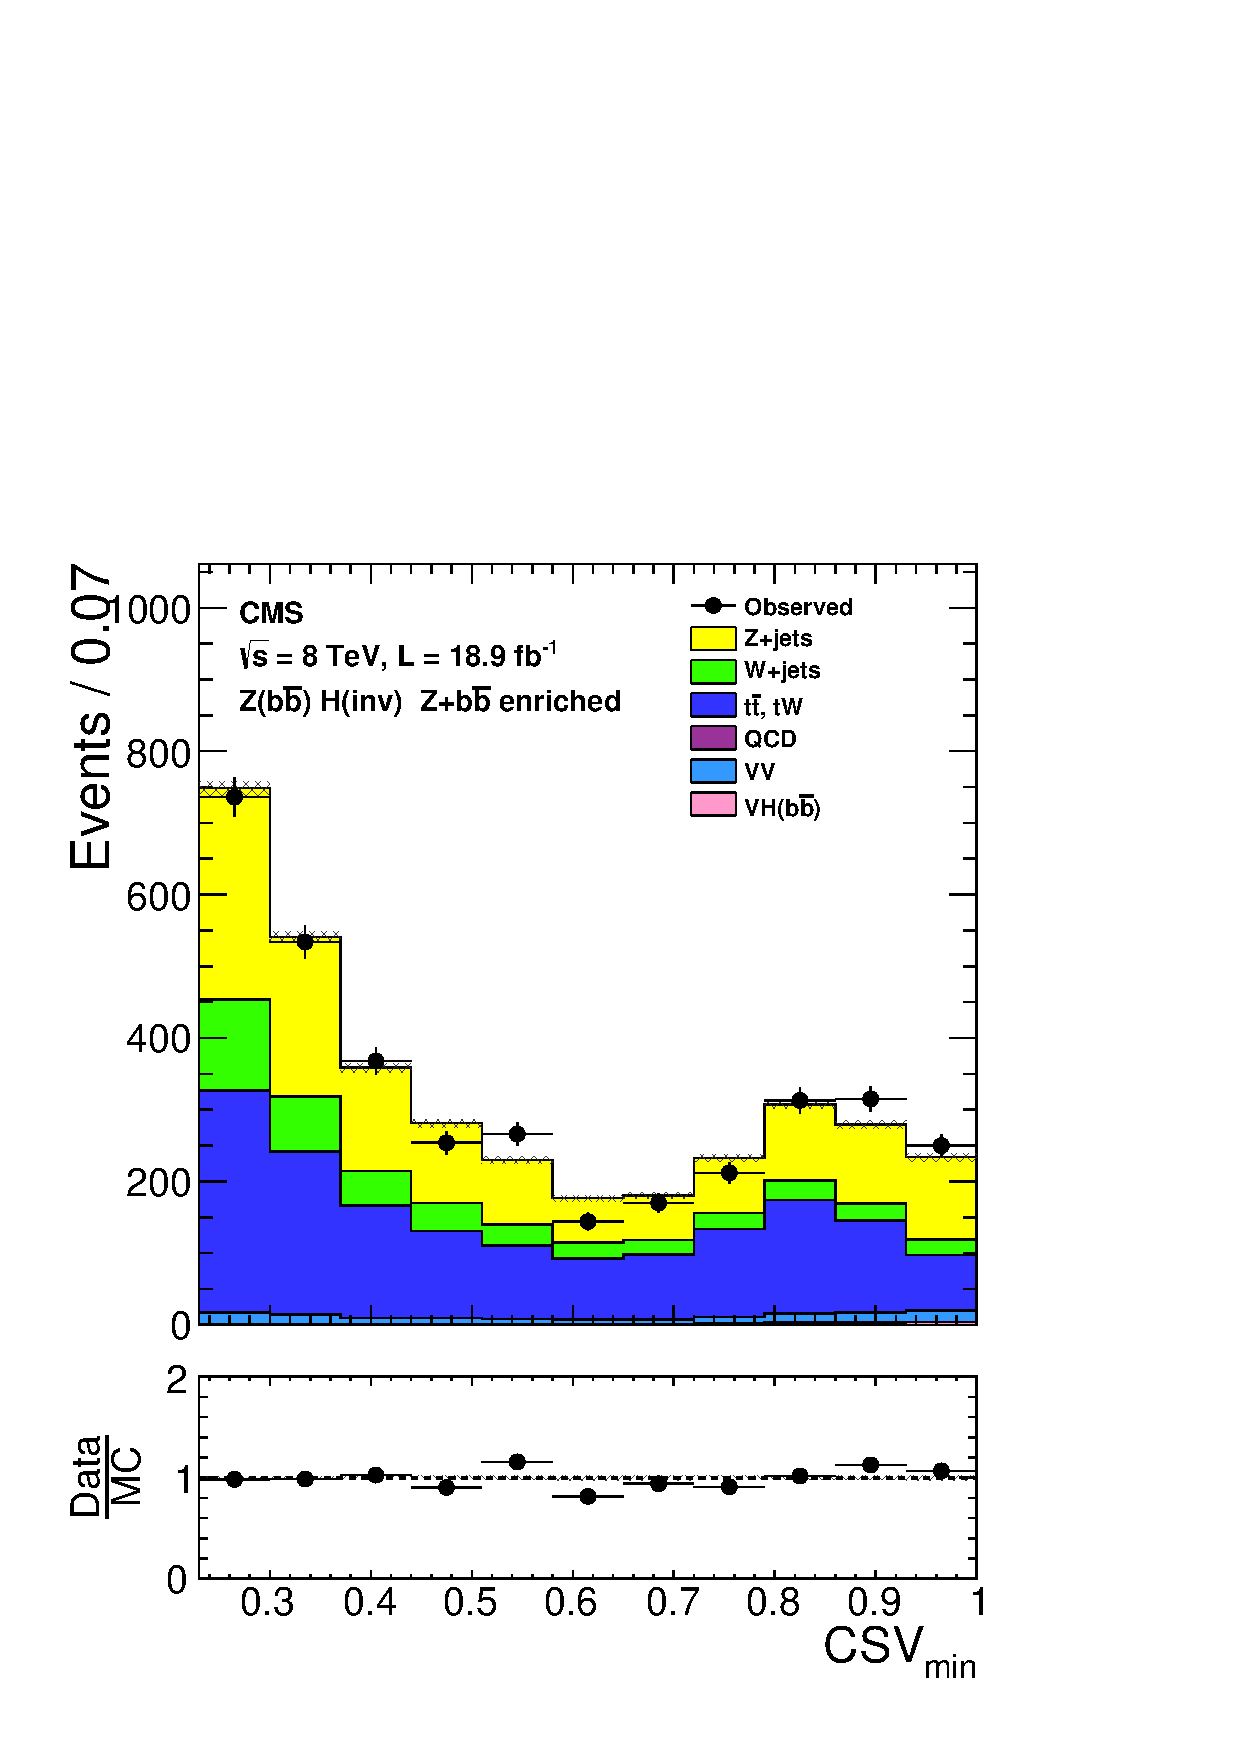
\includegraphics[clip=true,trim=0 0 0 20, width=.95\textwidth]{../invisible/TalkPics/panicpics/zbbcsv.pdf}
        \column{.1\textwidth}
        \hspace{-.4cm}\begin{turn}{-90}\scriptsize arXiv:1404.1344 \end{turn}
      \end{columns}
    \end{columns}


  \end{frame}

  \begin{frame}
    \frametitle{Z($b\bar{b}$)H results}
    \vspace{-.2cm}
    \begin{columns}
      \column{.7\textwidth}
    \begin{block}{}
      \centering
      \tiny
      \begin{tabular}{lccc}
        \hline
        Process & High $p_{T}(V)$ & Intermediate $p_{T}(V)$ & Low $p_{T}(V)$ \\
        \hline
        Total backgrounds & $181.3\pm 9.8$ & $64.8\pm 4.1$ & $40.5\pm 4.1$ \\
        Z($b\bar{b}$)H(inv) & $12.6\pm 1.1$ & $3.6\pm 0.3$ & $1.6\pm 0.1$ \\
        Observed data & 204 & 61 & 38 \\
        \hline
      \end{tabular}
    \end{block}
    \end{columns}
    \begin{columns}
      \column{.5\textwidth}
    \begin{block}{}
      \scriptsize
      \begin{itemize}
      \item Multivariate analysis (BDT):
      \item[-] performed for each mass hypothesis and boost region
        \scriptsize
      \item Limits from a fit to the BDT output distribution
       \item Assuming SM Higgs production cross-section and acceptance:
       \item[-]  observed(expected) 95\% C.L. limit on $B(H\rightarrow inv)$ for $m_{H}$=125 GeV is 182(199)\%
      \end{itemize}


    \end{block}
    \column{.5\textwidth}
    \begin{columns}
      \column{.95\textwidth}
      \vspace{.05cm}
      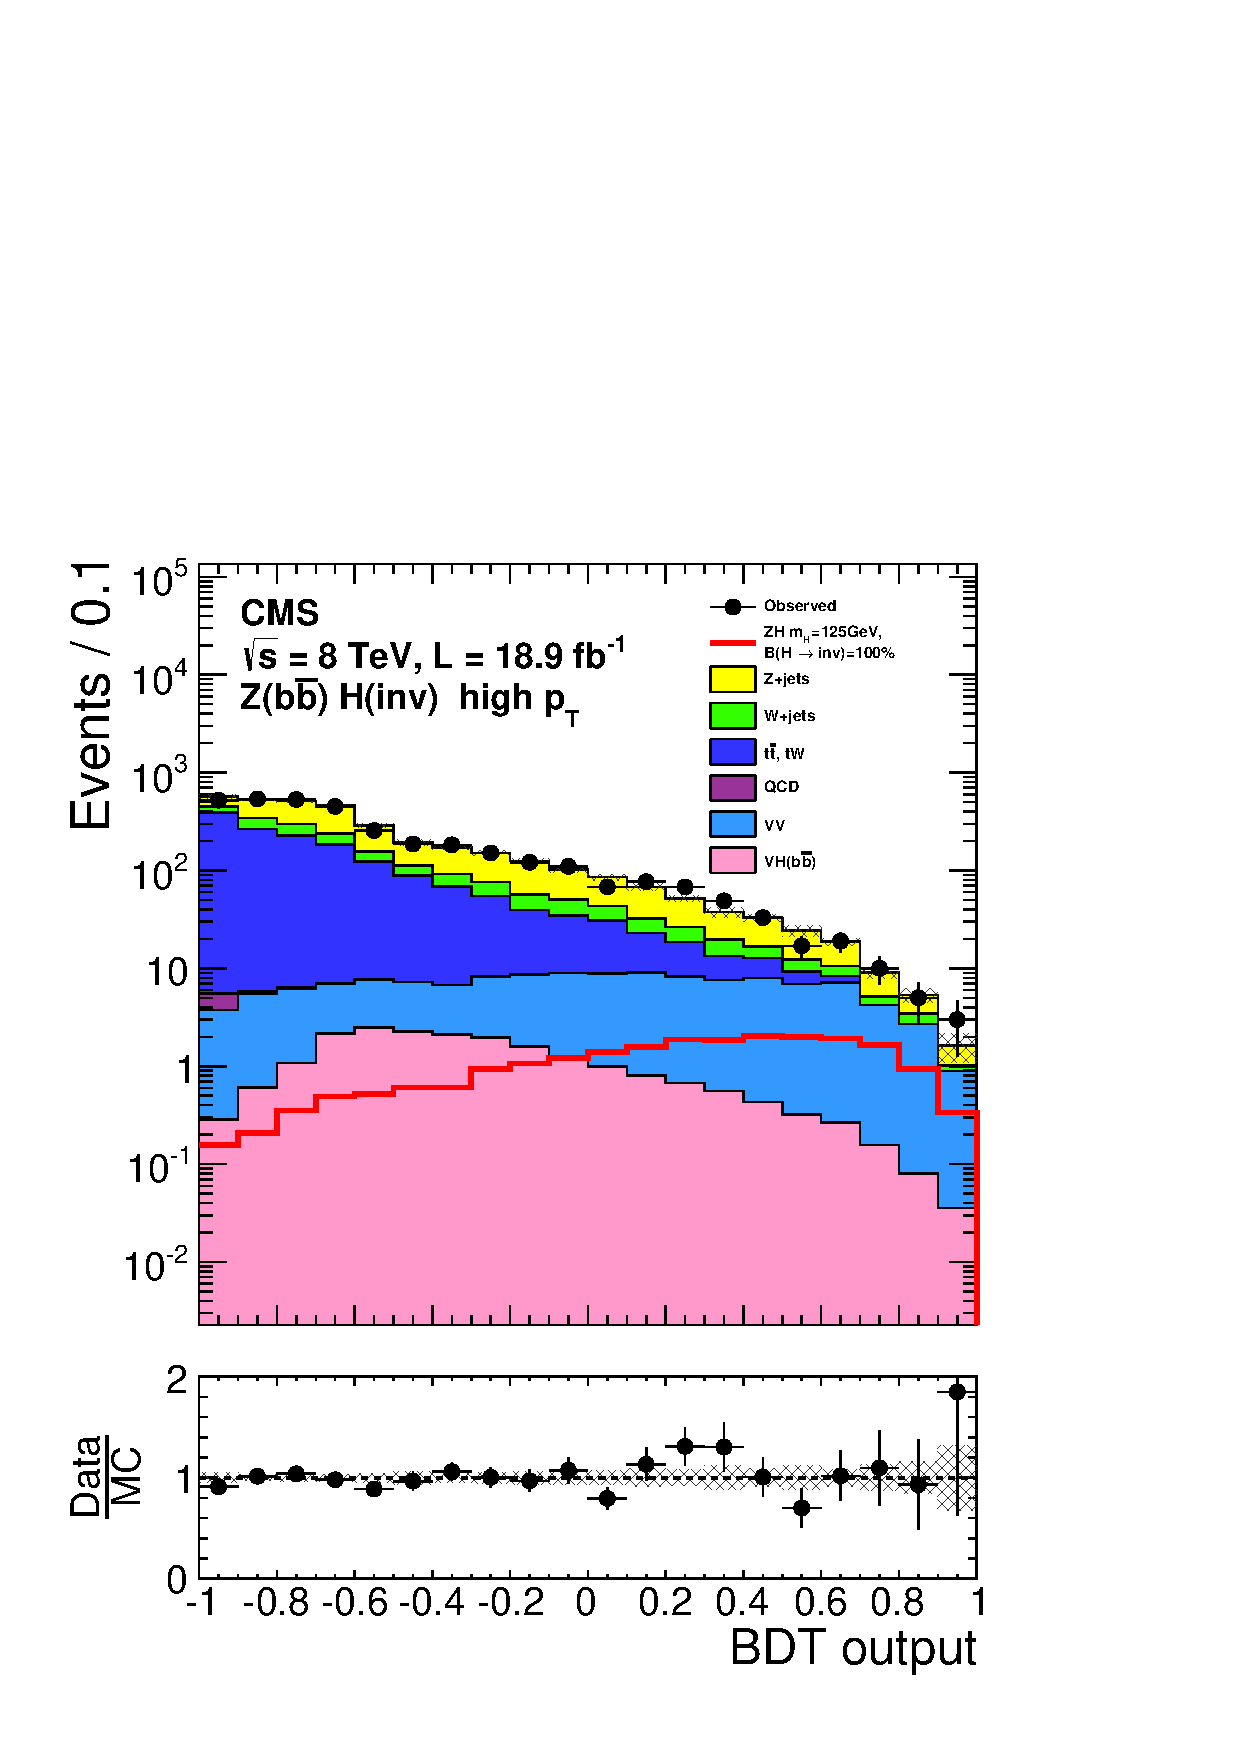
\includegraphics[clip=true,trim=0 0 20 0, width=\textwidth, height=.7\textheight]{../invisible/TalkPics/panicpics/zbbbdt.pdf}
      \column{.05\textwidth}
              \hspace{-.2cm}\begin{turn}{-90}\scriptsize arXiv:1404.1344 \end{turn}
    \end{columns}
    \end{columns}

      
  \end{frame}


  %% \begin{frame}
  %%   \frametitle{Other direct Limits}
  %%   \begin{block}{}
  %%     \begin{itemize}
  %%     \item ATLAS also produce a limit in the Z($\ell\ell$)H channel:
  %%     \item[-] observed (expected) 75\% (62\%) at 95\% C.L.
  %%     \end{itemize}
  %%   \end{block}
  %% \end{frame}
  
\end{fmffile}
\end{document}

